% 物理评论 B 97, 205409 (2018) 的中文翻译
% 原文：Emilia Ridolfi, Caio H. Lewenkopf, Vitor M. Pereira,
%       "Excitonic structure of the optical conductivity in MoS2 monolayers"
% 逐节对照翻译，公式编号、图号与原文献一致，参考文献保留原文。
\documentclass[11pt,a4paper]{ctexart}

\usepackage{amsmath,amssymb,bm}
\usepackage{graphicx}
\usepackage{booktabs}
\usepackage{float}
\usepackage{geometry}
\usepackage{xcolor}
\usepackage[colorlinks=true,linkcolor=blue!45!black,citecolor=blue!45!black,urlcolor=blue!45!black]{hyperref}
\geometry{margin=2.5cm}
\graphicspath{{figs/}}

\newcommand{\ii}{\mathrm{i}}
\newcommand{\eps}{\varepsilon}
\newcommand{\kk}{\mathbf{k}}
\newcommand{\kq}{\mathbf{k}'}
\newcommand{\qq}{\mathbf{q}}
\renewcommand{\thefootnote}{\fnsymbol{footnote}}

\begin{document}
\thispagestyle{empty}

\begin{center}
{\LARGE 单层 MoS$_2$ 光学电导率的激子结构}\\[2mm]
{\large Excitonic structure of the optical conductivity in MoS$_2$ monolayers}\\[5mm]
Emilia Ridolfi,$^{1}$\quad Caio H. Lewenkopf,$^{2}$\quad Vitor M. Pereira$^{1,3,*}$\\[2.5mm]
{\small
$^{1}$新加坡国立大学先进二维材料中心，6 Science Drive 2, Singapore 117546\\
$^{2}$巴西弗鲁米嫩塞联邦大学物理研究所，24210-346 Niterói, Brazil\\
$^{3}$新加坡国立大学物理系，2 Science Drive 3, Singapore 117542\\
$^{*}$通讯作者：vpereira@nus.edu.sg}
\end{center}

\vspace{1mm}
{\small\noindent 收稿 2018 年 1 月 24 日，修回 2018 年 4 月 18 日，发表 2018 年 5 月 8 日。\par}
{\small\noindent DOI: 10.1103/PhysRevB.97.205409\par}

\vspace{5mm}
\begin{center}
\textbf{摘要}
\end{center}
{\noindent
我们研究单层 MoS$_2$ 的激子谱，并计算其在很宽能量范围内的光学吸收性质。
我们的方法同时考虑二维体系的反常屏蔽与衬底的存在，两者都用一个合适的有效 Keldysh 势来描述。
我们用 Slater-Koster 紧束缚模型作为基组求解 Bethe-Salpeter 方程，
该模型的参数通过拟合从头算得到的 MoS$_2$ 能带确定。
由此得到的光学电导率在直到紫外能量范围内与已有测量结果在定量上吻合。
我们确认 C 激子的电子贡献并不来自 $\Gamma$ 点，而是来自布里渊区中大片区域上的一组 $k$ 点。
我们的结果进一步说明，基于有效模型的方法可以快速探索 TMD 体系激子的性质与可调控性。\par}

\vspace{8mm}

%=====================================================================
\section{引言}

块体三方相二硫化钼（MoS$_2$）来源广泛，这使得它成为研究得最充分的过渡金属硫族化合物（TMD）之一，
在严格的单层厚度下尤其如此，也把 MoS$_2$ 推到了石墨烯之外半导体二维材料家族中最受关注的位置 [1--5]。
与人们对样品制备与输运性质优化的持续兴趣和进展并行，MoS$_2$ 及与之密切相关的其它 TMD
在光电子应用上极具吸引力 [1,4,5]。
这推动了大量研究去理解支配这类晶体对光响应的物理过程。
在理解基本性质与探索这类材料在器件中的潜在用途两方面，理论与实验都取得了很大进展
[6--22] 与 [12,17,23--42]。

与几乎所有严格二维材料一样，MoS$_2$ 单层具有高度可调的载流子密度 [3,43--45]，
并且可以通过各种外部手段按需裁剪其性质，包括定制光学带隙 [46]。
人们很早就认识到，TMD 的本征二维性与半导体特征带来了增强的库仑相互作用，
它不仅重整化电子能带结构、对一切派生出的单粒子过程产生定量影响，
还在半导体光学响应中产生了迄今最强的激子效应 [47--49]。
其束缚能高达 0.22--1.1~eV [6,7,9--15,26,30--32,34]（具体数值取决于环境导致的相互作用强度），
并具有很大的谱重 [10,23,27]，这些双粒子激发决定了并主导了 TMD 材料的光学响应。
因此，激子现在被理解为任何可靠的 TMD 光学性质理论与模型中不可或缺的要素，
以至于任何不考虑激子效应的理论，连光学带隙与谱重分布最基本的定性特征都无法给出。

半导体 TMD 单层之所以有趣，还因为其电子结构具有若干独特性质，
这些性质可以拓宽其在光电子学中的适用范围。
例如，强自旋轨道（SO）耦合在 $K$ 点把价带劈裂了很大的量（$\Delta_{\mathrm{SOC}}$），
由此产生两族激子 [29]（见图 1(b) 中的 A、B 激子），
并允许选择性地激发具有预定自旋极化的电子 [50]。
此外，非零的 Berry 曲率提供了许多机会去探索与带边附近电子态的非平庸拓扑性质相关的应用，
包括通过光泵浦注入谷极化载流子 [51--54]、利用自旋-谷锁定同时控制自旋与谷布居 [55]，
以及由于拓扑起源的赝自旋轨道耦合导致的束缚激子能级的反常劈裂 [56,57]。

有鉴于此，发展足够灵活、能够预测 TMD 在不同实验条件下光学响应的可靠模型显然很有意义。
理想情况下，人们希望有一个方案，既能扩大精确且无偏的第一性原理全激子谱计算的适用范围，
又能提高其效率。
后者在数值上要求极高，而且对二维材料而言，要达到合理的收敛尤为繁重 [10,58]。
如果只依赖这类方法去扫描可能很大的修改范围（结构、化学、电子），
以针对特定目的裁剪材料的本征响应，就会变得代价过高。

\begin{figure}[H]
\centering
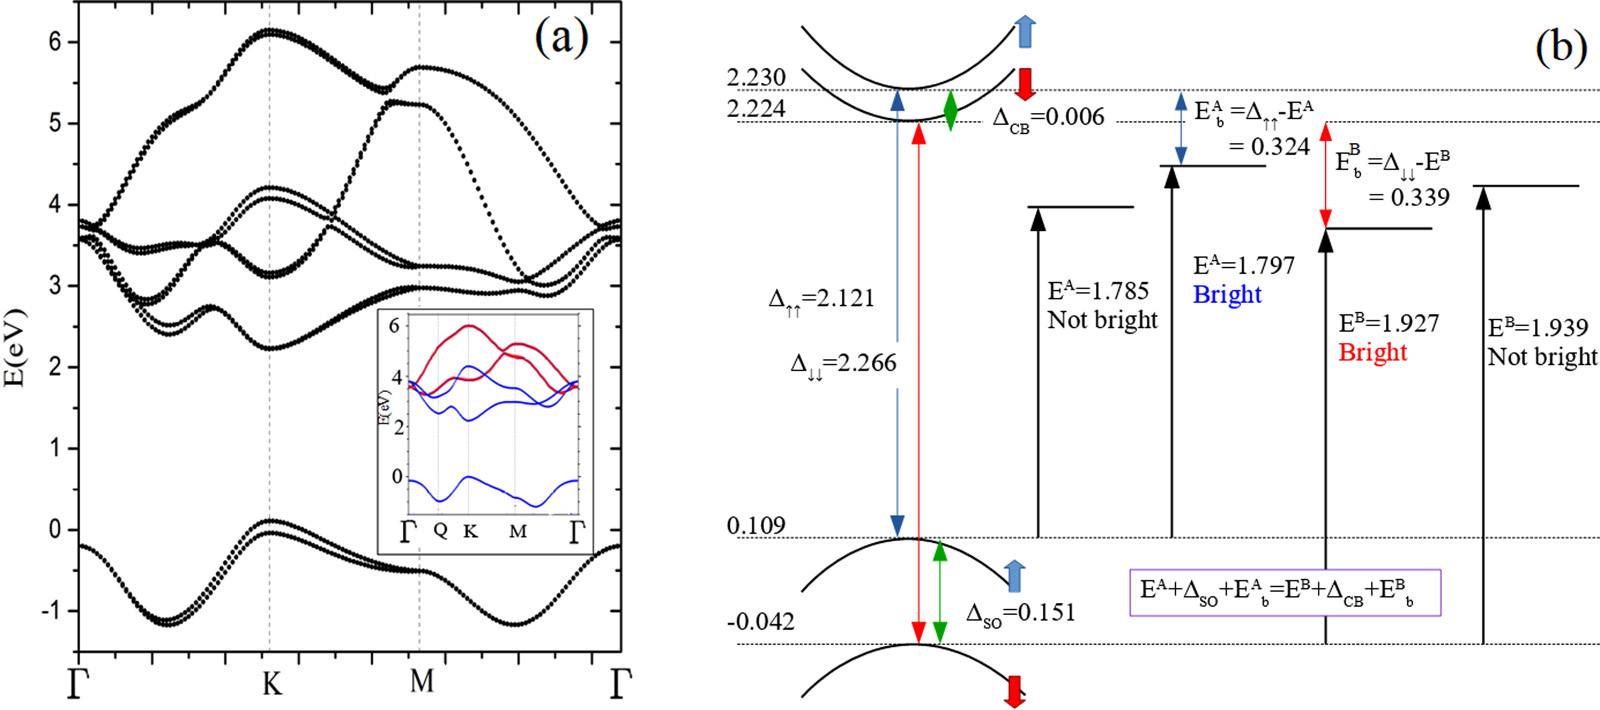
\includegraphics[width=1.0\textwidth]{fig1.png}
\caption{（原文 FIG.~1）(a) 按正文讨论、并已在文献 [59] 中报道的 Slater-Koster 参数化给出的 MoS$_2$ 单层参考能带结构（含 SO 耦合）。
整个模型哈密顿量可以按对 Mo 平面的反射对称性（$z$ 反射）解耦为奇、偶两个块。
插图是不含 SO 耦合的能带结构，其中偶（奇）宇称能带用蓝色（红色）标出。
(b) 基本带隙附近能量色散的示意（未按比例），以及与本工作激子谱相关的各个能量尺度，
包括由各激子系列导出的光学带隙（$E_{A,B}$）与激子束缚能（$E_b^{A,B}$）。
该图故意放大了 SO 耦合导致的导带 6~meV 劈裂，以便看清我们结果中每个系列出现两个不同激发能的来源
（例如图 3(a) 中的 $E_A$ 亮态与非亮态）。
实验上的 A、B 峰分别对应 $E_A$（亮）与 $E_B$（亮），图中各量满足 $E_A+\Delta_{\mathrm{SOC}}+E_b^{A}=E_B+\Delta_{\mathrm{CB}}+E_b^{B}$。}
\label{fig:1}
\end{figure}

本文关注单层体系。除非特别说明，下文把 MoS$_2$ 单层简称为 MoS$_2$。
我们描述的方法从对目标能带结构做精确的 Slater-Koster（SK）紧束缚参数化开始 [59]。
模型参数以第一性原理计算与实验信息为基准，用来描述 MoS$_2$ 最重要的谱特征，
例如布里渊区（BZ）各临界点上低能导带与价带的正确能量和轨道成分。
我们能在频率与绝对量级两方面定量再现实验测得的光学吸收谱。
正如预期，我们的计算与那些很好描述了强局域 A、B 激子的已有理论工作 [6,9,10,31,60] 一致。
通过在布里渊区中对 $k$ 点做大量采样，我们还能够研究所谓 C 激子 [10] 并确定其性质，
这正是文献中仍在争论的问题 [10,28,31,33]。

本文其余部分安排如下：第~II~节讨论 TMD 单层光学响应的实验与理论现状。
第~III~节给出我们用针对 MoS$_2$ 单层优化的 SK 哈密顿量求解 BSE、
并据此计算线性响应光学电导率的方法。
第~IV~节讨论结果，重点是共振 C 激子的性质。第~V~节总结主要结论。
文中还包含一个附录，讨论若干技术问题，例如计算中能带条数的选择、
光学响应中自旋轨道效应的分析，以及有无库仑相互作用时能谱的对比。

%=====================================================================
\section{MoS$_2$ 光学响应中的激子}

少层与单层 MoS$_2$ 的光学电导率、吸收与反射谱已在近期实验中被广泛研究 [12,23--33]。
现在已经确认，干净、未掺杂单层的光吸收起始于 $1.8\pm0.1$~eV，
这一结论来自反射与光致发光光谱 [12,23,24,27,31,32]、吸收谱 [26--28,33]、
光电子能谱 [29] 以及二次谐波分析 [35,38,39]。
吸收阈值处有两个相距 $145\pm4$~meV 的峰 [29]，
它们对应由自旋劈裂的价带与导带之间跃迁产生的两族激子（A 与 B）。
角分辨光电子能谱 [12] 以及 X 射线光电子能谱与扫描隧道显微/谱 [34] 的研究表明，
单粒子带隙位于 2.15--2.35~eV 之间，由此给出最低 A 激子的束缚能为 0.22--0.42~eV
（需要注意，吸收峰存在不可忽略的温度依赖，这是提取束缚能、判断实验差异时的重要因素 [17,61--63]）。
如此大的束缚能意味着异常小的激子半径，典型值约为 5~\AA{} [13]，但仍属 Wannier-Mott 型。

在理论方面，基于 GW 修正电子态的第一性原理 BSE 解能够准确抓住与 A、B 激子相关的实验行为
[6,9,10,31,60]。但这些工作也暴露出全从头算方法在二维体系中的数值困难：
无论 GW 单粒子修正阶段还是随后的 BSE 求解，收敛都极为苛刻 [9,10,31,58,60,65]。
另一方面，有效模型必须处理屏蔽势的非库仑形式，
这对正确描述束缚激子系列是必需的 [66--68]，却使束缚能与波函数无法写成解析形式。
用适配 MoS$_2$ 的大质量 Dirac 方程描述导带谷与价带谷的 $k\cdot p$ 模型 [9,14,26,50]
已经能够抓住束缚激子系列 [9,14,26]、激子谱的动量色散 [13]，
以及激子对光学电导率的贡献 [15,26,50]。
这类模型研究的一个普遍特点是只关注特定特征，最典型的是能谱本身，
后者是非氢型的 [16,57,66]，直到近期才被正确描述。
这种受限的分析是有效质量方法的隐含要求，但对基于紧束缚的模型并不构成限制：
只要起始哈密顿量能定量准确、定性忠实地描述单粒子态，
紧束缚模型就能描述整个布里渊区以及与实验和应用相关的大能量范围。
参数化模型，无论是 SK 型还是更简单的、不区分轨道的紧束缚哈密顿量，
都已被采用，精度与对实验的再现程度各不相同 [7,11,13,15]：
有的只报告 A、B 峰附近有限能量范围的结果 [7,13]；
有的采用拟合参数很多（例如超过 28 个）的紧束缚模型 [11,13]，
或者只用 $d$ 轨道基组 [13,15]（远离 $K$ 点时轨道成分会变得重要，
例如文献 [10] 把 C 激子指认为同时具有 Mo $d_{z^2}$ 与 S $p_{x,y}$ 成分的态）。
更重要的是，其中一些计算的单粒子能带结构无法很好抓住 GW 修正后的带隙 [13]
或高导带的色散 [14]，而这些恰恰是激子问题中特别相关的因素。

最后要指出，由于所涉及的电子激发具有零晶体动量，
块体 MoS$_2$ 光学性质中的激子特征在定性与定量上都与单层相似。
这源于块体的层状结构：层间电子耦合相对较弱，
使得块体的电子性质在很大程度上有强烈的二维特征。
因此并不奇怪，尽管屏蔽环境不同，块体样品中的激子束缚能与半径往往与单层相近 [69]，
并且仍主要局域在单层之内 [8]。
所以理解单层中的激子物理，是描述块体中相应物理的关键。

%=====================================================================
\section{理论与方法}
\subsection{激子态与 BSE}

晶体中的中性激发，无论束缚态还是扩展态，都可以用 BSE 的近似解很好地描述 [58,70--73]。
在此框架下，第一性原理方法已被广泛用于研究绝缘体与半导体的光学性质，
并成为处理固体材料激子谱的现行标准 [58]。
库仑相互作用与屏蔽是激子问题的核心，必须以自洽的方式妥善处理，
才能确立体系的“单粒子”基态（即其单粒子能带结构）。
除求解 BSE 本身之外还需要自洽地计入准粒子修正，
这在实现与计算时间两方面都是显著挑战。
因此，对 MoS$_2$ 激子谱及相关可观测量的彻底且收敛的第一性原理计算历来少而稀疏 [9,10,31,60]。

既然激子物理对描述半导体 TMD 的光学响应不可或缺，
而目前又需要既准确又快速的方法来处理这些性质，
我们用一个正交的 SK 紧束缚哈密顿量求解 BSE 并计算光学电导率，
该哈密顿量的参数化用来描述 MoS$_2$ 的能带结构。
原子轨道基组包括每个 S 原子的三个 $p$ 价轨道以及每个 Mo 原子的五个 $d$ 轨道，
在三方晶胞内共 11 个原子轨道。
哈密顿量的构造与 SK 参数优化的细节已在别处给出 [59]。简要地说，其主要特征是：
(i) 只有 14 个拟合参数；(ii) $K$ 点处正确的 2.115~eV 带隙；
(iii) $K$ 点价带 150~meV 的自旋劈裂；
(iv) $K$、$\Gamma$ 以及所谓 Q 点处导带与价带的有效质量与位置。
SO 耦合的紧束缚参数选取为让 $\Delta_{\mathrm{SOC}}$ 与实验上 A、B 峰的能量差相符 [29]。
相应的能带结构复制于图 1(a)，反映出洁净单层的绝缘基态。
由该哈密顿量得到的 Bloch 态 $\psi_{n\mathbf k}(\mathbf r)$ 被视为晶体哈密顿量本征态的良好近似，
\begin{equation}
\hat H\,\psi_{n\mathbf k}(\mathbf r)=\eps_{n\mathbf k}\,\psi_{n\mathbf k}(\mathbf r),
\end{equation}
其中
\begin{equation}
\psi_{n\mathbf k}(\mathbf r)=\frac{1}{\sqrt{N_c}}\sum_{\mathbf R}e^{\ii\mathbf k\cdot\mathbf R}
\sum_{\alpha}C^{n}_{\alpha,\mathbf k}\,\varphi_{\alpha}(\mathbf r-\mathbf R-\mathbf t_{\alpha}).
\end{equation}
晶格矢量 $\mathbf R$ 取遍晶体的全部 $N_c$ 个原胞，$n$ 是能带指标，
$\alpha$ 标记轨道，$\mathbf t_{\alpha}$ 是轨道中心在晶胞内的位置。
能带指标 $n$ 与轨道指标 $\alpha$ 都取同一区间 $[1,N]$，
其中 $N=22$（$11\times2$，含自旋）是 SK 哈密顿量所用轨道基的维数。
这些 Bloch 态用来在 Tamm-Dancoff 近似（TDA）下建立 BSE：
引入费米海的双粒子激发基，
\begin{equation}
|\mathrm{FS}\rangle\equiv\prod_{v\mathbf k}a^{\dagger}_{v\mathbf k}|0\rangle,
\qquad
|v\mathbf k\to c\mathbf k\rangle\equiv a^{\dagger}_{c\mathbf k}a_{v\mathbf k}|\mathrm{FS}\rangle .
\end{equation}
后者用来展开激子态
\begin{equation}
|M\rangle=\sum_{c,v,\mathbf k}A^{M}_{cv\mathbf k}\,|v\mathbf k\to c\mathbf k\rangle,
\end{equation}
能量记为 $E_M$，$M$ 标记各激子模式。
需要注意，这些定义隐含地把激子动量限制为零；这足以抓住所有一阶光学过程，
因为零动量激子才是光学亮态。
因此下文只讨论这一子空间。
此外沿用“c/v”的传统记号表示导带与价带，以强调我们处理的是零温情形。
此处还需指出，由于 $c\in[1,N_c]$、$v\in[1,N_v]$，
其中 $N_c$、$N_v$ 分别是导带与价带的条数，
式 (3) 中基态张成的向量空间维数为 $N_{\mathrm{tot}}\equiv N_k^2\times N_c\times N_v$，
$N_k^2$ 表示布里渊区内采样的总点数。
即便在参数化的紧束缚框架内，能带条数与 $k$ 点采样规模仍是双粒子谱计算的关键限制因素之一。

把式 (4) 代入包含多体库仑相互作用的薛定谔方程，
得到约化本征问题 [11,13,74]
\begin{equation}
E_{cv\mathbf k}A^{M}_{cv\mathbf k}
+\frac{1}{V}\sum_{c'v'\mathbf k'}W_{cv\mathbf k,c'v'\mathbf k'}A^{M}_{c'v'\mathbf k'}
=E_M A^{M}_{cv\mathbf k},
\end{equation}
其中 $E_{cv\mathbf k}\equiv\eps_{c\mathbf k}-\eps_{v\mathbf k}$ 是 $c$、$v$ 两条带在 $\mathbf k$ 处的能量差，
$V\equiv A_cN_k^2$ 是晶体总面积
（$A_c=\sqrt3a^2/2$，$a\simeq3.16$~\AA{} 为晶格常数），
$W_{cv\mathbf k,c'v'\mathbf k'}\equiv\langle v\mathbf k\to c\mathbf k|\hat U|v'\mathbf k'\to c'\mathbf k'\rangle$
是多体库仑势 $\hat U$ 在两个粒子-空穴激发之间的矩阵元。
在 TDA 下该矩阵元包含直接项与交换项两部分 [75]。
如文献 [13] 早先指出的，在正交基组下、且在我们所设的库仑作用与状态轨道成分无关的近似下，
交换项对零动量激子没有贡献。
因此只剩直接库仑矩阵元，可以简单地写成 [11,13]
\begin{equation}
W^{(d)}_{cv\mathbf k,c'v'\mathbf k'}=u(\mathbf k-\mathbf k')\,
I^{*}_{c'\mathbf k',c\mathbf k}\,I_{v'\mathbf k',v\mathbf k},
\end{equation}
其中 $u(\mathbf q)$ 是屏蔽库仑势的傅里叶变换 [58]。
定义 SK 基组时假设的正交性 [59] 使我们能把交叠积分 $I_{a\mathbf k',b\mathbf k}$
用 Bloch 态 (2) 的展开系数表示：
\begin{equation}
I_{a\mathbf k',b\mathbf k}=\sum_{\alpha}C^{a*}_{\alpha\mathbf k'}\,C^{b}_{\alpha\mathbf k}.
\end{equation}
由于 $C^{b}_{\alpha\mathbf k}$ 来自 Bloch 哈密顿量的数值本征矢，
必须保证相位选取一致，因为 $I_{a\mathbf k',b\mathbf k}$ 不是规范不变量。
我们要求波函数在基组上的系数之和 $\rho_{\mathbf k n}=\sum_\alpha C^{n}_{\alpha\mathbf k}$ 为实数，
这也是文献 [58] 的建议。

%---------------------------------------------------------------------
\subsection{屏蔽库仑相互作用}

准确描述式 (6) 中的屏蔽库仑相互作用，对真实再现激子谱至关重要 [58]。
早期从理论上描述 MoS$_2$ 及相关二维材料激子系列的工作正好说明了这一要求的严格：
若简单地采用裸库仑势，就无法抓住实验观测到的非里德伯能级结构 [16,57,66]。
MoS$_2$ 中分立的束缚激子能级序列既源于其赝自旋自由度 [16]，
也源于严格二维电子体系中改变了的静电相互作用，后者在动量空间中具有如下形式 [66,67]
\begin{equation}
u(q)=-\frac{e^2}{2\eps_0\eps_d\,q\,\kappa(q)},
\qquad \kappa(q)\equiv1+r_0q ,
\end{equation}
其中 $r_0$ 定义电子体系的二维极化率 [65--67]，
$\eps_d$ 描述 MoS$_2$ 单层上下介质带来的静态均匀屏蔽 [12]。
我们假设有效厚度为 $d$、有效介电常数为 $\eps_2$ 的 MoS$_2$ 单层夹在介电常数为 $\eps_1$ 与 $\eps_3$ 的材料之间，
环境介电常数因此为 $\eps_d=(\eps_1+\eps_3)/2$。
式 (8) 正是 Keldysh 为薄金属膜导出的形式，此时参数 $r_0$ 相当于膜厚 [68]。
介电函数 $\kappa(q)$ 中由多体相互作用带来的显式 $q$ 依赖，
定性地改变了实空间中的库仑定律，使其变为
\begin{equation}
u(r)=-\frac{e^2}{8\eps_0\eps_d r_0}
\left[H_0\!\left(\frac{r}{r_0}\right)-Y_0\!\left(\frac{r}{r_0}\right)\right],
\end{equation}
其中 $H_0$ 与 $Y_0$ 分别是 Struve 函数与 Bessel 函数。
参数 $r_0$ 定义一个交叉长度尺度，把 $\propto1/r$ 的长程衰减与
$r\to0$ 时以 $\propto\log r$ 奇异性为特征的短程区域分开 [65]。
从头算研究已确认 Keldysh 相互作用能准确描述 MoS$_2$ 中的屏蔽势 [9,76]。
因此我们在式 (6) 中采用 $u(q)$ 来求解 BSE。

现在只剩 $r_0$ 与 $d$ 两个参数需要确定，才能完全指定式 (5) 的内容。
近期文献中它们在不同作者之间的报道差异很大 [9,12--14]。
二维极化率的从头算给出真空中 $r_0\sim31.2$--$41.5$~\AA{} [9]。
然而已知激子能级序列的精确能量位置对单层周围介电环境的细节很敏感 [13,15,18,46]。
针对空气/衬底界面介电环境下单层的既有估计给出一个较宽的区间，
即 $r_0\sim13.55$--$57.6$~\AA{} [9,12--14]。
由于我们以 Li 及其合作者 [27] 的测量作为实验光学电导率的参照，
取环境介电常数 $\eps_d=2.5$，这正适合空气/二氧化硅界面（$\eps_1=1$，$\eps_3=4$）。
在目前还没有从头算给出二氧化硅衬底对极化率修正的情况下，
我们沿用文献 [12,13] 基于 Keldysh 型有限厚度（$d$）模型给出的估计：
\begin{equation}
r_0=\frac{2\eps_2^2-\eps_1^2-\eps_3^2}{2\eps_2(\eps_1+\eps_3)}\,d .
\end{equation}
其中 $\eps_2$ 表示 MoS$_2$ 的有效介电常数。
取 [12] $d\simeq6$~\AA{}、$\eps_2\simeq12$（后者与块体 MoS$_2$ 介电常数的第一性原理结果相符 [9]）
时与实测激子束缚能符合得最好，由此得到 $r_0=13.55$~\AA{} [77]。

在这样指定了全部贡献之后，尽管近期已提出数值上更高效的方法 [11]，
我们仍通过对式 (5) 的本征问题做完全对角化来求解 BSE。
考虑到当前实验覆盖的能量范围，我们把式 (3) 中的基态限制为
$N_v=2$ 条价带（因显式包含自旋，实际为 $1\times2$）与 $N_c=8$ 条导带之间的激发。
需要注意，在 $k\cdot p$（Dirac）近似下考虑有效模型时，
必须在有效薛定谔方程中额外引入赝自旋自由度才能正确描述能谱 [16]。

%---------------------------------------------------------------------
\subsection{光学响应}

$D_{3h}$ 点群决定了所有二阶张量在面内是各向同性的，
因此在 MoS$_2$ 单层中只需考虑光学电导率的对角分量 $\sigma(\omega)\equiv\sigma_{xx}(\omega)$，
它在偶极近似、$T=0$ 下的线性响应为 [11,78]
\begin{equation}
\operatorname{Re}\sigma(\omega)=\frac{e^2\pi}{m^2\hbar\omega V}
\sum_M\left|\langle\mathrm{FS}|\hat P_x|M\rangle\right|^2
\delta(\omega-\omega_M).
\end{equation}
用式 (4) 表示 $|M\rangle$，可把总动量算符的矩阵元写成
\begin{equation}
\langle\mathrm{FS}|\hat P_x|M\rangle
=\sum_{cv\mathbf k}A^{M}_{cv\mathbf k}
\langle\mathrm{FS}|\hat P_x\,a^{\dagger}_{c\mathbf k}a_{v\mathbf k}|\mathrm{FS}\rangle .
\end{equation}
按通常方式展开多体动量算符 $\hat P_x=\sum_{pq}\langle p|\hat p_x|q\rangle a^{\dagger}_pa_q$，有
\begin{equation}
\langle\mathrm{FS}|\hat P_x\,a^{\dagger}_sa_r|\mathrm{FS}\rangle
=\sum_{pq}\langle p|\hat p_x|q\rangle
\times\left[\delta_{pr}\delta_{qs}f_r(1-f_s)+\delta_{pq}\delta_{sr}f_pf_s\right],
\end{equation}
其中 $f_j$ 是电子在态 $j$ 上的费米-狄拉克占据数。
在零温下，并注意我们关心的是 $c\ne v$ 的情形，可写成
\begin{equation}
\langle\mathrm{FS}|\hat P_x\,a^{\dagger}_{c\mathbf k}a_{v\mathbf k}|\mathrm{FS}\rangle
=\langle\psi_{v\mathbf k}|\hat p_x|\psi_{c\mathbf k}\rangle
=\frac{m}{\hbar}\langle\psi_{v\mathbf k}|\nabla_{k_x}\hat H(\mathbf k)|\psi_{c\mathbf k}\rangle .
\end{equation}
把式 (2) 给出的 Bloch 态代入，光学电导率 (11) 变为
\begin{equation}
\operatorname{Re}\sigma(\omega)
=\frac{e^2}{4\hbar}\frac{4\pi}{\hbar\omega V}
\sum_M\Biggl|
\sum_{\alpha\beta}\sum_{\mathbf k cv}A^{M}_{cv\mathbf k}
C^{v*}_{\alpha\mathbf k}C^{c}_{\beta\mathbf k}
\Biggl.\langle\varphi_\alpha|\nabla_{k_x}\hat H(\mathbf k)|\varphi_\beta\rangle
\Biggr|^2\delta(\hbar\omega-\hbar\omega_M).
\end{equation}
这一形式明确显示：每个粒子-空穴激发的振子强度既依赖 BSE 的解（$A^{M}_{cv\mathbf k}$），
也依赖晶体动量表象下有效哈密顿量的成分（$C^{c}_{\alpha\mathbf k}$）。

无相互作用（单粒子）近似下的响应可直接得到：
没有粒子-空穴相互作用时，BSE 即式 (5) 是对角的。
在此极限下 $A^{M}_{cv\mathbf k}\to\delta_{cv\mathbf k,M}$、$E_M\to E_{cv\mathbf k}$，
式 (15) 简化为
\begin{equation}
\operatorname{Re}\sigma_{\mathrm{sp}}(\omega)
=\frac{e^2}{4\hbar}\frac{4\pi}{\hbar\omega V}
\sum_{\alpha\beta}\sum_{cv\mathbf k}\Biggl|
C^{v*}_{\alpha\mathbf k}C^{c}_{\beta\mathbf k}
\Biggl.\langle\varphi_\alpha|\nabla_{k_x}\hat H(\mathbf k)|\varphi_\beta\rangle
\Biggr|^2\delta(\hbar\omega-E_{cv\mathbf k}).
\end{equation}

%=====================================================================
\section{结果}
\subsection{激子谱的收敛性}

我们用沿倒格矢 $\mathbf b_1=(2\pi/a,\,2\pi/a\sqrt3)$、$\mathbf b_2=(2\pi/a,\,-2\pi/a\sqrt3)$
所定义方向上的 $N_k$ 个均匀采样点来求解式 (5) 的本征问题。
把 $\Gamma$ 点放在原点，$K$ 与 $M$ 位于所取布里渊区采样域的中心（见下文图 5(a)）。
由于库仑相互作用在倒空间中并不周期，而我们的方法又不包含局域场项（即第一布里渊区之外的傅里叶分量），
采样域的选择会影响束缚激子能级的能量，
尤其是当这些能级来自布里渊区边界附近 $k$ 点的跃迁时。
更具体地说，式 (5) 中对 $\mathbf k'$ 的求和形式上覆盖整个倒空间，
可以写成 $\mathbf k'\equiv\mathbf k''+\mathbf Q$，其中 $\mathbf k''$ 取遍第一布里渊区，$\mathbf Q$ 为倒格矢。
当激子波函数强烈局域在布里渊区边缘时，必须计入 $\mathbf Q\ne0$ 的项，
否则就会漏掉处于相邻布里渊区、波矢相近的 $k$ 态之间的重要库仑矩阵元。
由于与本问题相关的波函数局域在布里渊区中各 $K$ 点附近（下文将讨论，见图 5），
我们只保留 $\mathbf Q=0$（即只考虑第一布里渊区内的全部波矢与矩阵元），
所得到的激子谱即可收敛，并与文献 [27] 报道的实验一致。
能够在不影响谱收敛的前提下做这样的库仑矩阵元截断，为计算的数值效率带来额外改进。

不过要注意，任何离散化方法都需要对 $k$ 对角矩阵元 $W_{cv\mathbf k,c'v'\mathbf k}$
做正则化，因为屏蔽势的长程尾巴导致 $\propto1/|\mathbf k-\mathbf k'|$ 的可积奇异性（参见式 (8)）。
由于它们对式 (5) 的贡献在热力学极限 $N_k\to\infty$ 下变得正则，
这种正则化在如下意义上是良定义的：具体做法在该极限下对计算结果没有影响。
但我们发现，正则化方案会显著影响谱随 $N_k$ 的收敛速度，
在给定的收敛目标下可以把 Bethe-Salpeter 矩阵的维数降低一个数量级。
这一点在实践上很重要，因为在我们这样的有效 SK 描述中，
能带条数按构造就是先验所需的最小集合，
于是布里渊区采样成为决定数值问题规模与可解性（对给定计算精度而言）的限制因素。
由于奇异矩阵元要在 $k$ 空间上积分，最直接的正则化做法是把 $u(\mathbf q=\mathbf k-\mathbf k'=0)$
替换为它在包含原点的小区域 $\Delta q$ 上的平均值，即
\begin{equation}
u(\mathbf q\approx0)\to\frac{1}{\Delta q}\int_{\Delta q}u(\mathbf q)\,\mathrm d\mathbf q
\approx\frac{c\,aN_k}{2\pi}
\times\left[\alpha_1+\alpha_2\frac{2\pi r_0}{aN_k}
+\alpha_3\left(\frac{2\pi r_0}{aN_k}\right)^2\right],
\end{equation}
其中 $c\equiv-e^2/(2\eps_0\eps_d)$，常数 $\alpha_j$ 取决于平均区域 $\Delta q$ 的几何形状
以及展开式 (17) 的截断阶数。

\begin{figure}[H]
\centering
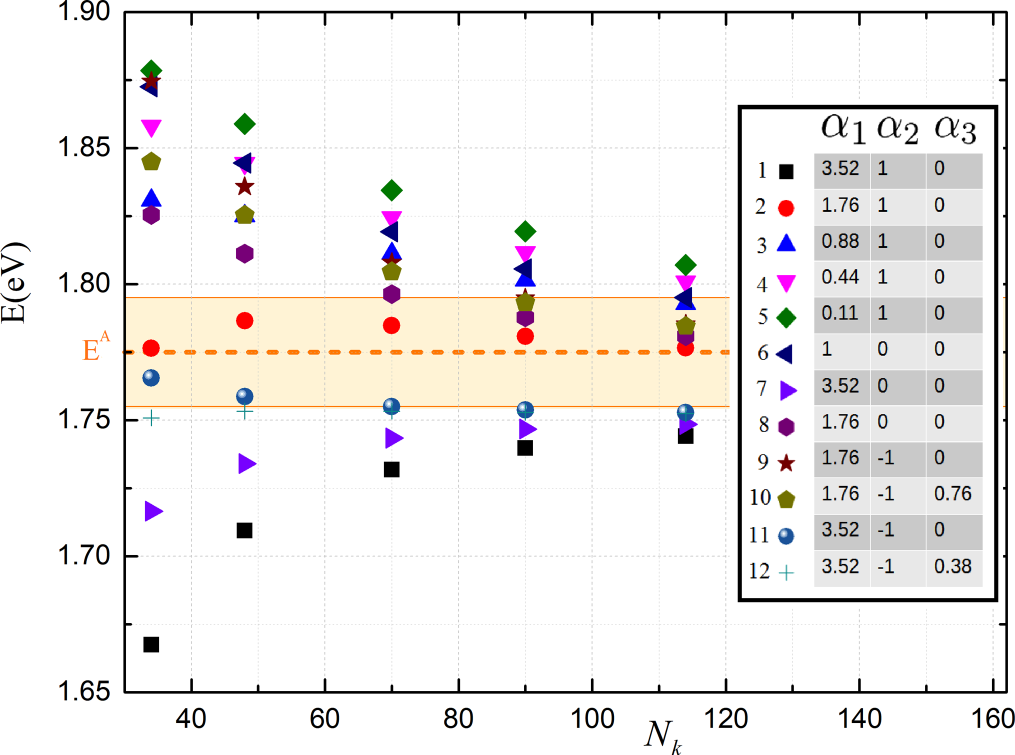
\includegraphics[width=0.7\textwidth]{fig2.png}
\caption{（原文 FIG.~2）BSE 最低本征值的能量（$E_A=1.775$~eV，暗态，参见图 3(a)）
随布里渊区均匀采样总点数 $N_k$ 的变化。
水平虚线表示对不同正则化方案下所有曲线做联合外推得到的值。
阴影带标出外推结果 $\pm20$~meV 的能量区间。}
\label{fig:2}
\end{figure}

图 2 展示了最低激子能级（$E_A$）随采样规模变化的不同收敛速率。
为演示起见，这些数据是在只保留每种自旋离带隙最近的两条能带（即 $N_c=N_v=2$）下求解式 (5) 得到的。
可以清楚看到，某些正则化方案能更快地逼近渐近值。
特别地，若在展开式 (17) 中忽略更高阶项、取 $\alpha_1=1$、$\alpha_{2,3}=0$
（参数组 \#6，见图 2 标注），收敛特别慢 [79]。
这并不意外，因为 $2\pi r_0/a\simeq26.9$，恰好与实际可达到的 $N_k$ 量级相同 [80]。
相反，参数组 \#2 与 \#11（见图 2 标注）收敛快得多，
能在 0.020~eV 精度内收敛到渐近值 $E_A=1.775$~eV [81]。
由于我们的 SK 能带参数化中单粒子带隙为 $E_g=2.12$~eV [59]，
这对应束缚能 $E_b^A=0.34$~eV
（该值对应第一个暗 A 激子；第一个亮激子为 $E_A=1.80$~eV，束缚能 $E_b^A=0.32$~eV）。
此后所有计算都按正则化方案 \#2 给出。我们已验证它对整个谱都有效。

图 3(a) 把由 BSE 得到的本征值与二氧化硅中 MoS$_2$ 在单粒子带隙范围内的实验谱 [27,30] 做了直接比较。
我们发现，除了 0.07~eV 的全局刚性偏移之外，
用我们的模型参数得到的谱极好地再现了束缚激子系列。
特别地，它准确抓住了最低几个态的能级间距，而这些态正是对短距离下修正后的屏蔽势 (9) 最敏感、
因而偏离氢型谱最明显的态 [16,57,66]。
该谱还再现了基态激子为暗态这一近来由实验确认的事实 [82]。
对最低的几个激子态，我们得到约 12~meV 的亮-暗劈裂。
这一数值来自自旋轨道耦合导致的导带 6~meV 间距以及有效质量差异。
我们的结果与其它理论计算一致，后者在 20~meV 左右 [83--85]，具体取决于从头算方法的类型。
迄今为止，对 MoS$_2$ 中亮-暗劈裂唯一的直接实验研究 [82] 给出约 100~meV。
考虑到理论文献以及自旋轨道耦合更强的 TMD（如 MoSe$_2$、WSe$_2$）中观测到的 47--57~meV [82,86]，
这一数值大得有些意外。
这些迹象表明，MoS$_2$ 中亮-暗劈裂的定量方面仍处于实验检验之中。

\begin{figure}[H]
\centering
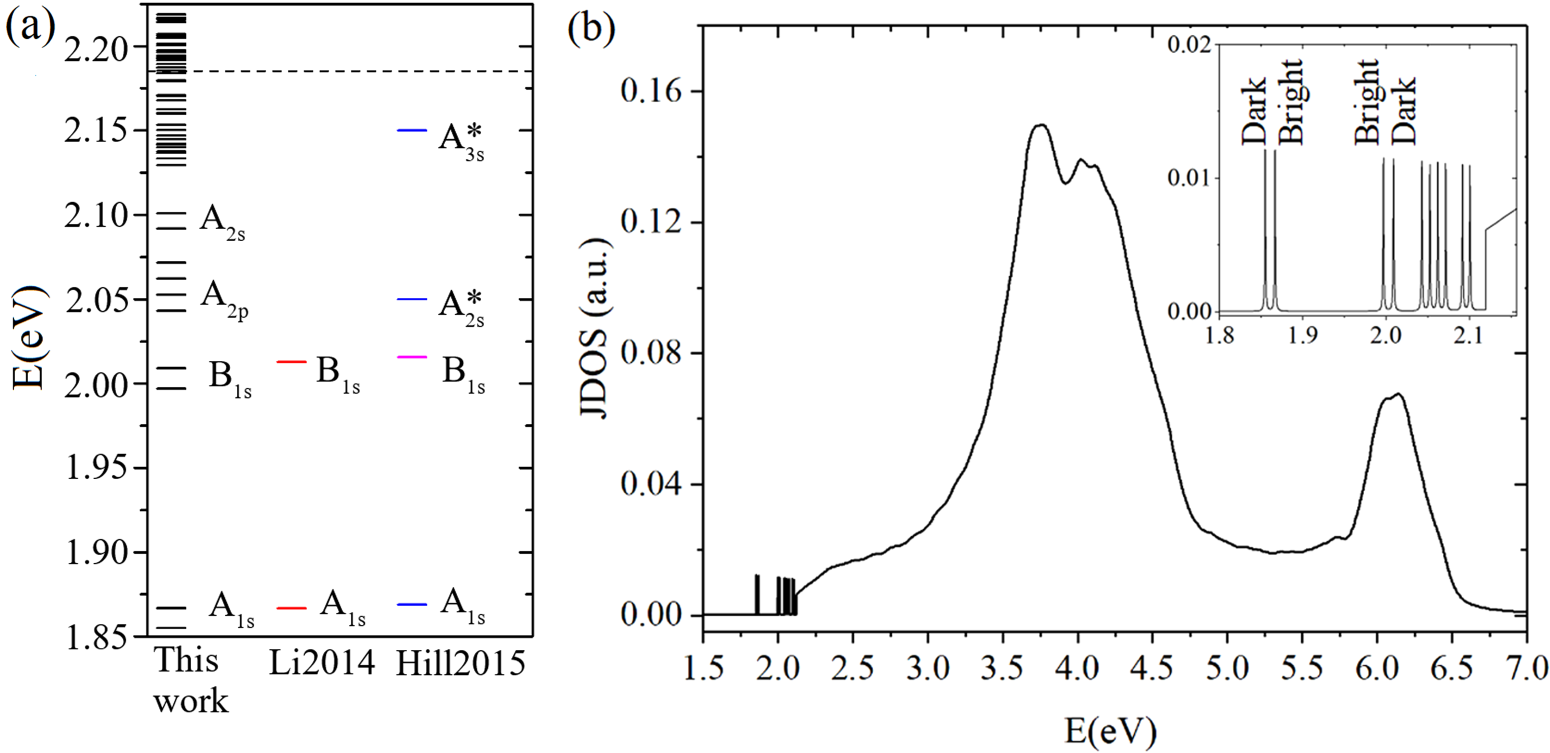
\includegraphics[width=1.0\textwidth]{fig3.png}
\caption{（原文 FIG.~3）(a) 本工作得到的理论激子谱低能部分与文献 [27,30] 测得的 A、B 峰能量的比较
（注意文献 [30] 中对标记为 $A_{2s}^*$、$A_{3s}^*$ 的峰指认并不唯一）。
把能量整体刚性移动 $+0.07$~eV（见正文）之后，理论谱极好地再现了实验 A、B 峰的位置。
水平虚线表示 2.18~eV 处的单粒子能隙（$2.18=2.12+0.07$）。
(b) 按式 (18) 定义的激子联合态密度，已整体移动 $+0.07$~eV。
所用洛伦兹展宽的全宽为 0.1~eV，但在低能区（插图中放大显示）取 0.001~eV，以便分辨单个束缚激子能级。}
\label{fig:3}
\end{figure}

为便于把吸收谱与实验直接比较，图 3 所示结果中已把能量做了 $+0.07$~eV 的刚性蓝移。
这种“标定”在某种程度上是可预期的，因为能带结构与屏蔽库仑势都采用了有效参数化 [87]
（不过与同类方法中需要多达 0.57~eV 的修正 [13] 相比，0.07~eV 的偏移算很小）。
这一能量轴的标定同样用于我们此后所有结果的展示。

束缚系列直接对应布里渊区 $K$ 点附近最高价带与最低导带之间的跃迁。
由于 $K$--$K'$ 谷简并，每个能级都是二重简并的。
若忽略 $K/K'$ 处两条最低自旋极化导带之间的小能量差，还会多出一重二重简并。
在我们的计算中，这个小的能量差显式地为有限值（参见图 1(b)），
这解释了图 3(a) 中例如标为 $A_{1s}$ 的两个靠得很近的能级的来源。
不过要记住，由于宇称选择定则，这些激子中只有一半是光学亮态 [13]。

在这一点上值得指出：最低束缚 A、B 激子的激发能之差并不严格等于能带的自旋轨道劈裂。
这一点很重要，因为文献中许多紧束缚参数化直接把 $E_B-E_A$ 等同于 SO 耦合参数，
等价地，这一激子劈裂也常被当作单粒子能带中自旋轨道劈裂的直接实验度量，而这并不严格正确。
例如我们得到 $E_B-E_A=130$~meV，而所选紧束缚模型中由 SOC 导致的价带劈裂为 150~meV。
这一差别主要可追溯到自旋劈裂的两条价带具有不同的有效质量 [7]。

为确定能保证整个谱收敛的 $k$ 点采样，我们分析了激子联合态密度（JDOS），
\begin{equation}
\rho_J(E)\equiv\frac{1}{N_cN_vN_k^2}\sum_M\delta(E-E_M),
\end{equation}
其中 $E_M$ 是 BSE 的本征值。
计算表明，$N_k=48$ 时 JDOS 已相当收敛，而 $N_k=90$ 到 120 之间差别可以忽略。
本文给出的结果取 $N_k=60$。
图 3(b) 给出 $N_k=60$、$N_c=8$ 条导带与 $N_v=2$ 条价带下收敛的 JDOS。

%---------------------------------------------------------------------
\subsection{线性光学电导率}

线性阶的光学电导率可由式 (15) 与 (16) 直接得到：
在上述 10 条能带张成的子空间中、对布里渊区做合适采样，
把完整的 BSE 矩阵对角化即可。
狄拉克 $\delta$ 函数用全宽为 $\gamma$ 的洛伦兹函数代替以引入展宽。
$\gamma$ 定性地代表若干微观机制造成的总衰减率，
每种机制都以各自特征的能量依赖贡献于 $\gamma$ [10]。

\begin{figure}[H]
\centering
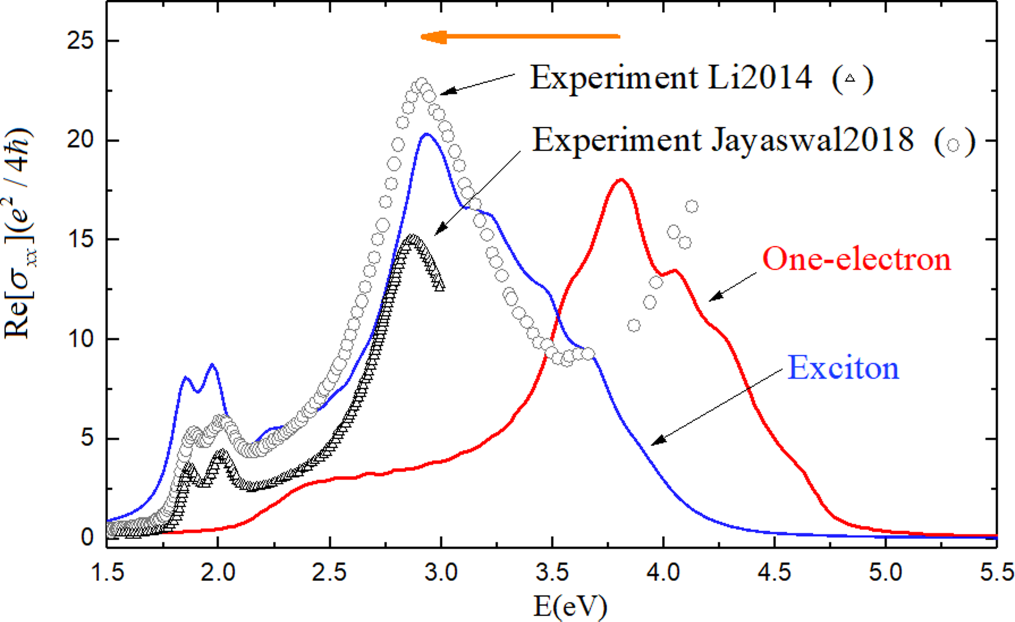
\includegraphics[width=0.75\textwidth]{fig4.png}
\caption{（原文 FIG.~4）文献 [27] 与 [88] 报道的室温下二氧化硅上 MoS$_2$ 单层线性光学电导率实验曲线（黑色），
与我们含（蓝色）与不含（红色）粒子-空穴相互作用的结果对比（$N_c=8$，$N_v=2$，$N_k=60$）。
计算得到的 $\sigma(\omega)$ 额外加了 0.136~eV（全宽）的能量无关洛伦兹展宽，
以反映实验上 A、B 激子处的展宽。高能处衰减到零是人为的：
BSE 对角化所用能带条数有限，使计算谱只在约 3.5~eV 以下完整。
尽管如此，为完整起见这里仍给出这些能带所覆盖的整个范围。}
\label{fig:4}
\end{figure}

由于实验展宽在很大程度上依赖无序与样品，我们采取简单做法：把 $\gamma$ 视为常数，
调整其数值去拟合实验数据（见下文讨论）。
图 4 给出单粒子与 BSE 计算得到的 $\sigma(\omega)$ 实部，这是我们最重要的结果。
作为参照，图中还画出了 Li 等人 [27] 对剥离 MoS$_2$、
以及 Jayaswal 等人 [88] 对 CVD 生长 MoS$_2$ 近期报道的实验曲线，两者都在室温下的二氧化硅上测得。
需要注意，与实验数据的比较只在约 3.5~eV 以下有意义，
更高能量处必须计入本文计算未包含的其它价带参与的激发（图 1(a)）[59]。
计算中取 $\gamma=0.068$~eV，对应 Li 等人实验中 A、B 激子峰的平均宽度。
正如预期，单粒子结果无法描述光学响应的谱特征。
尽管偏差在束缚激子能级主导的区域（$E\lesssim2.1$~eV）最明显，
连续区里也存在显著差别。
特别地，单粒子谱重总体上分布在远高于相互作用修正后数值的能量处，
如图 4 中的水平箭头所示。
因此，若忽略激子效应、把单粒子吸收谱照字面理解，
就会在光学带隙附近乃至整个能量范围造成严重的定性与定量失真。
可见这些二维材料中的强库仑相互作用不仅导致高激子束缚能，还大幅重整化了整个谱。

图 4 显示我们的 BSE 计算相当好地抓住了 MoS$_2$ 光学电导率的重要实验特征，
即 A、B 峰的位置、在 $E_C\simeq2.85$~eV 处的整体极大值、
整个实验范围内的能量依赖，以及光学电导率的绝对量级。
要强调，我们并没有调整或缩放 $\sigma(\omega)$ 的量级，
而这类做法在讨论类似实验对比的理论工作中很常见。
这种整体吻合证明了底层能带结构的 SK 参数化的有效性与准确性，
也强有力地支持了在 BSE 计算中使用 Keldysh 有效屏蔽势
（近期文献中不同理论与实验谱的进一步汇总见图 7）。
由于 $\gamma$ 对应依赖激发能的微观过程，人们可能会预期这种依赖对光学电导率的线形有明显影响。
然而我们用常数展宽的计算已相当令人满意地再现了测得的能量依赖。
出乎意料的是，从头算结果 [10,31,60] 尽管计入了具体的能量依赖展宽过程（如电子-声子散射 [10]），
对 $\operatorname{Re}\sigma(\omega)$ 的描述反而不如我们准确（见图 7(b)）。
这表明实验展宽很可能由无序主导，也事后证明了我们选用能量无关的 $\gamma$
去展宽式 (15) 中数值离散谱的合理性。

最后，如文献 [10] 所指出的，做到大 $k$ 网格的收敛研究，
对于有意义地“再现 2 eV 以上实验吸收谱的特征”是必需的。
图 7 的对比很好地说明了：在效率与需要大布里渊区采样以保证收敛这两方面，
基于参数化 SK 模型的方法可以优于 BSE 的全第一性原理求解。
当然，关键在于所依赖的底层能带结构从一开始就要准确描述准粒子重整化。

%---------------------------------------------------------------------
\subsection{C 激子的性质}

$\operatorname{Re}\sigma(\omega)$ 在 $E_C$ 处的极大值曾被归因于
涉及布里渊区中心（$\Gamma$ 点）附近跃迁的共振激子，即所谓 C 激子 [10]。
如下文将讨论的，这些激子与 $\Gamma$ 点的关联其实并不比与 $K$ 点的更强。
因此把它们称作“$\Gamma$ 点激子”是不正确的。
关注 $E_C$ 附近电导率的谱细节，图 4 显示：
激子计算在 $[2.5,3.5]$~eV 区间给出的能量依赖，
几乎与单粒子计算在 $[3.5,4.5]$~eV 区间给出的相同。
这似乎表明，在该能区内电子相互作用的主要效果是把单电子电导率整体红移约 0.9~eV，
而线形没有显著改变（图 4 中水平箭头所指）。
若果真如此，把这一宽区域内增强的谱重归因于相互作用效应就值得怀疑，因为
(i) 单电子曲线似乎已经具备了 $\sigma(\omega)$ 能量依赖与量级的关键特征；
(ii) 激子修正除了把曲线整体移到低能（这正是吸引性电子-空穴相互作用所预期的）之外，
似乎并未产生任何新的谱特征。
换句话说，对于属于单粒子连续区的激发能，
相互作用对吸收谱的重构看起来相当于对能谱做一次“剪刀”型修正，
即用一个约 0.9~eV 的有效“束缚能”把单电子曲线（红）移到正确位置（蓝），而振子强度基本不变。
然而问题在于，0.9~eV 远大于 A 束缚激子的束缚能（$E_b^A=0.324$~eV）。
事实证明，用这些单电子能带结构特征来解释这一激子红移是有问题的，
而且正如我们下面详细说明的，过于简单且有误导性。

单电子曲线（图 4 中红色）在其极大值附近的大谱重，
主要来自最低导带沿 $\Gamma$-$K$ 的下行色散（见图 1）：
相隔约 4~eV 激发能的导带与价带彼此大致平行地色散，
会使该区域的单粒子 JDOS 大幅增强，自然解释了 $\operatorname{Re}\sigma(\omega)$ 的峰。
等价地，从图 1 可以看出，在我们的 SK 模型中，
单电子“光学能带结构”沿 $\Gamma$-$K$ 线几乎是平的。
因此单电子的“C 峰”主要是约 4~eV 处大 JDOS 的结果
（附录图 10 明确证实了这一点）。
然而同样的结论并不适用于激子计算的结果。
正如在图 3(b) 中所见，激子 JDOS 大致在约 4~eV 处成峰，
而相应的电导率却在 $E_C\simeq2.85$~eV 处成峰。
由此可见，$E_C$ 附近增强的光学响应显然不是大量能量接近 $E_C$ 的激子能级造成的。
实际上，除了在带隙中出现的束缚激子能级之外，
单粒子与激子 JDOS 在连续区的能量上差别不大，这一点我们在附录图 10 中演示。
例如，仅凭激子谱（通过 JDOS）来预测光学电导率的谱形，
在连续区能量上显然会失败。
这就是为什么前面讨论的“用约 0.9~eV 的有效束缚能把单电子谱整体红移”这一想法具有误导性。

因此必须显式考虑振子强度，按式 (15) 它由下式给出
\begin{equation}
\sum_{\mathbf k cv}A^{M}_{cv\mathbf k}
\sum_{\alpha\beta}C^{v*}_{\alpha\mathbf k}C^{c}_{\beta\mathbf k}
\left\langle\varphi_\alpha\left|\nabla_{k_x}\hat H(\mathbf k)\right|\varphi_\beta\right\rangle .
\end{equation}
回想 $A^{M}_{cv\mathbf k}$ 是激子 $M$ 在倒空间中的概率幅，
振子强度不仅取决于单电子偶极矩阵元，还取决于每个激子波函数在 $k$ 空间的具体纹理。

图 5 分析了与最大光谱重相对应的若干代表性激子波函数（参见图 4，另见图 6）。
正如前面关于能量“标定”的说明，各面板中标出的数值相对 BSE 的原始本征值
分别移动了 $+0.07$~eV（右栏）与 $+0.57$~eV（左栏）。
作为参照，图 5(b) 与 5(c) 表明与 A、B 激子相关的波函数集中在 $K$ 点附近 [89]，
这与以往计算早已确立的结论一致。
它们的局域程度直接与大束缚能相关，在实空间中它们比半导体中的典型激子局域得多 [5,13]。
回顾一下，由于宇称选择定则，跨在带隙两侧的两条价带与两条导带所涉及的激子中，
只有一半是光学亮态。
由于 $K$--$K'$ 谷简并，每个光学亮激子都是二重简并的
（当忽略 $K/K'$ 处两条最低自旋极化导带之间的小能量差时，
它们还与另一对二重简并的暗激子进一步简并；
在我们的计算中，这个小能量差显式地为有限值，与图 3 所示的谱相对应）。

对 C 激子而言情形相当不同。
图 5 面板 (d) 至 (g) 给出的波函数对应能量接近 $E_C$ 的若干选定态。
需要提醒读者：与 A、B 这类束缚激子不同，这里展示的是一个“连续谱”中若干代表性波函数
（我们在 $E_C$ 附近的能量窗口内核查过，
波函数像这样散布在布里渊区某些区域上是稳健的共同特征）。
显然我们所用的两个紧束缚模型 [13,59] 给出不同的态。
不过可以注意到，相应的波函数表现出相当大的相似性（比较图 5 的左右两栏）。
值得注意的是，$\Gamma$ 点本身并没有明显贡献；
相反，对我们所取的初基胞而言，激子波函数大致分布在一个环上，
该环与所有对称点都保持有限距离，位于 $K$-$M$ 与 $\Gamma$-$K$ 的中途。
这与在 C 激子区域对 BSE 做完全从头算求解所得的类似观察一致：
那些工作同样把 C 激子与类似环状区域内的跃迁联系起来，而非具体在 $\Gamma$ 处或附近 [10,31,90]
（例如见文献 [90] 的图 21）。
此外，图 5 中的 C 激子在 $k$ 空间中看起来比对应的 A 激子局域得更紧，
因为这些环相当细（同时也要记住色标是对数的）。
这种局域程度可以通过计算每个激子波函数的逆参与比在定量层面确立，我们在附录中给出。

\begin{figure}[H]
\centering
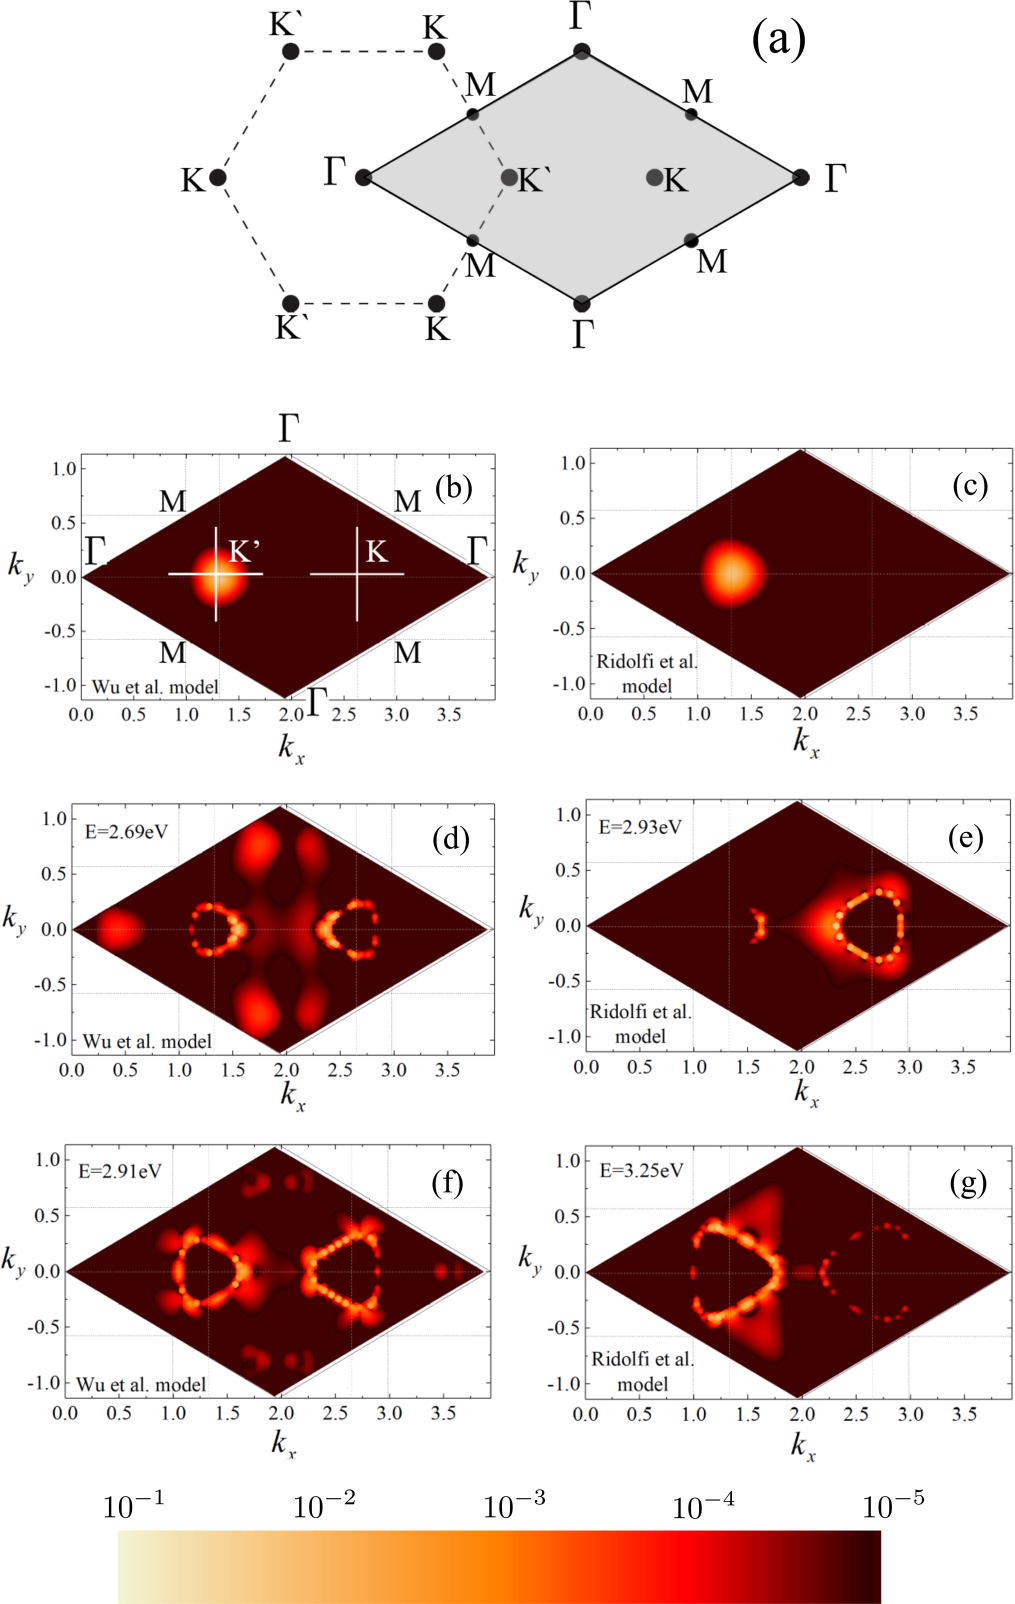
\includegraphics[width=0.45\textwidth]{fig5.png}
\caption{（原文 FIG.~5）动量空间中的代表性激子波函数，只包含离 $E_F$ 最近的两条导带与两条价带
（$N_k=60$，$N_c=N_v=2$）。
(a) MoS$_2$ 第一布里渊区（虚线）与我们在 $k$ 采样中使用的等价倒格原胞（实心菱形）示意图。
$\Gamma$ 点位于采样域的顶点处，$M=(\pi/a,-\pi/\sqrt3a)$，$K'=(4\pi/3a,0)$，$K=(8\pi/3a,0)$。
左栏为用文献 [13] 的紧束缚模型得到的波函数，右栏用文献 [59] 的 SK 参数化。
第二行 [(b)、(c)] 给出与光学电导率中 A 峰相关的某个波函数对应的概率分布密度图。
底部两行 [(d)--(g)] 给出 C 激子区域内的代表性波函数。坐标轴单位为 \AA$^{-1}$。色标为对数。}
\label{fig:5}
\end{figure}

\begin{figure}[H]
\centering
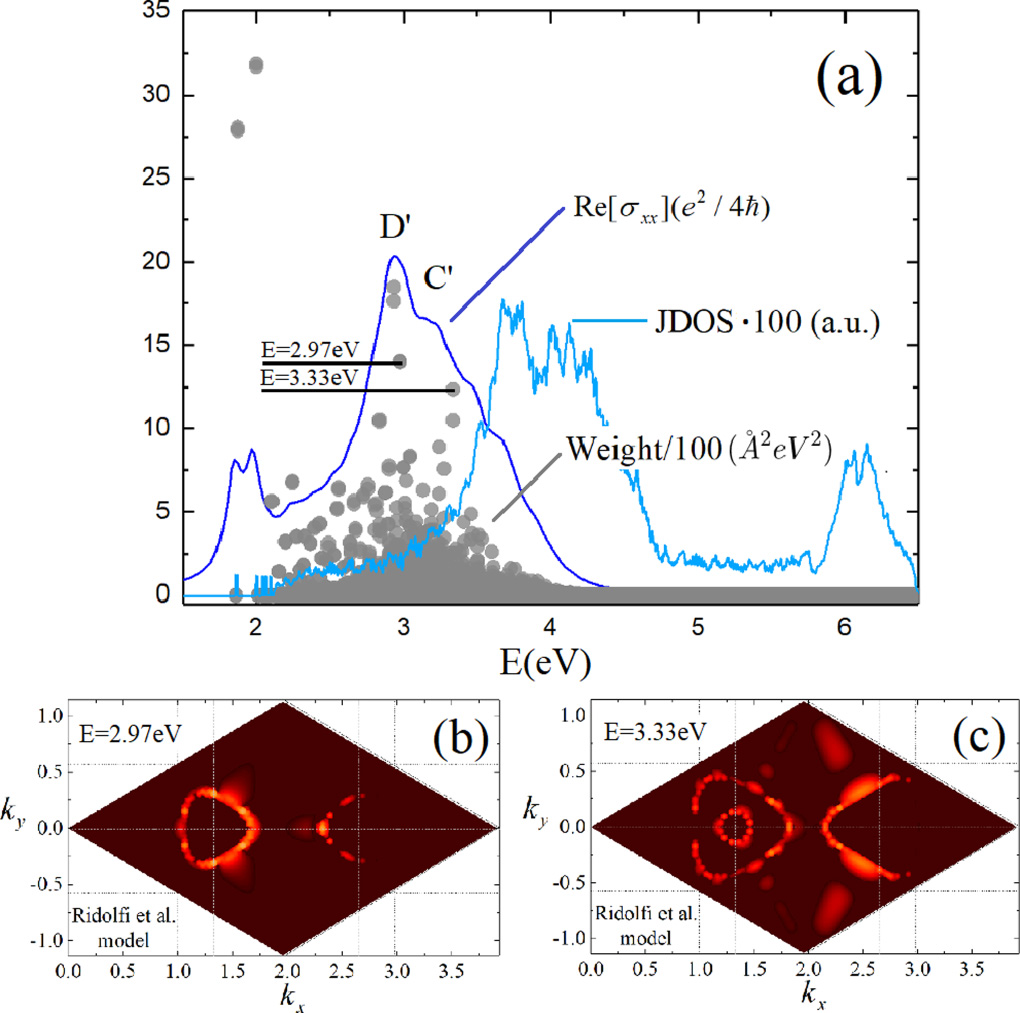
\includegraphics[width=0.55\textwidth]{fig6.png}
\caption{（原文 FIG.~6）(a) 按我们的激子计算，把光学电导率实部、激子 JDOS 与
式 (19) 给出的振子强度画在一起。
(b)、(c) 给出对 $D'$ 与 $C'$ 两个峰有贡献的代表性激子波函数，
它们的能量与光谱重已在 (a) 中标出（$N_k=60$，$N_c=8$，$N_v=2$）。坐标轴单位为 \AA$^{-1}$。
色标为对数，与图 5 相同。}
\label{fig:6}
\end{figure}

附录图 10(b) 的数据表明：C 激子所在区域的 JDOS 相对较小，
而相应的态通常比平均更局域 [91]。
这最终决定了振子强度的能量依赖，使它在 $E_C$ 附近的能区取极大，
从图 6 可以直接看出（该图对全部激子画出了式 (19) 所示的量）。
因此，与单粒子计算的情形相反，$\operatorname{Re}\sigma(\omega)$ 的谱形几乎完全由振子强度而非光学 JDOS 决定。

总之，上述讨论表明把这些激子称为“$\Gamma$ 点激子”是具有误导性的，
并强化了把它们与沿 $\Gamma$-$K$ 和 $K$-$M$ 方向的“光学能带结构”性质联系起来的视角 [10,31]。
把图 5 中激子波函数的计算从最低两条导带推广到我们紧束缚模型中的全部八条导带，
我们就可以确定地把振子强度中 $E\simeq2.9$~eV 与 $E\simeq3.3$~eV 的两个峰
（图 6 中标为 $D'$、$C'$）指认为文献 [33] 所区分的两种贡献。
具体地说，用我们的能带结构，它们来自沿 $\Gamma$-$K$ 与 $K$-$M$ 对称线
相距约 3.8~eV 的近似平行能带之间的粒子-空穴激发。
从这个角度看，属于宽 C 区域的激子确实具有约 0.9~eV 的大束缚能（$0.9=3.8-2.9$）。
值得注意的是，比较图 5(g) 与图 6(c) 会发现后者在靠近 $K$ 的内环上还有额外权重。
这部分来自价带到第五、第六条导带的跃迁，
这些导带在 $K$ 附近向下色散，彼此近似平行，间距约 4~eV。
这生动说明：对与整个 C 激子区域相关的精细细节的指认，
对底层能带结构的细节很敏感，必须计入更高的导带。

C 激子来自倒空间中 $\Gamma$-$K$ 与 $K$-$M$ 线中途的粒子-空穴激发，
这与 C 峰比 A、B 特征对薄 MoS$_2$ 膜的层数更敏感相一致。
特别地，$E_C$ 的实验移动与 MoS$_2$ 厚度引起的能带间距变化相关 [28,31,92]。
已知这些电子结构变化在 $K$ 点很小，而在整条 $\Gamma$-$K$ 线上很大，
最终决定了随厚度由直接带隙向间接带隙的转变 [24]。
A/B 与 C 激子之间的这种反差可以从以下事实理解：
$K/K'$ 处的电子态主要由 Mo 的 $d$ 轨道贡献，
而对 C 激子有贡献的 $k$ 区域则具有来自硫原子的强 $p$ 特征 [59,90,93]。
由于 $d$ 轨道在空间上更局域，而且位于构成每个 MoS$_2$ 单层的三个原子面之中间层，
与因强硫轨道成分而变化的 C 激子相比，
$K/K'$ 处的 A、B 激子态在堆叠多层结构或应变下受到的扰动要小得多 [90]。

%=====================================================================
\section{总结}

我们重新审视了单层 MoS$_2$ 激子谱的计算问题。
已经表明，与单粒子图像相比，多体效应在异常宽的能量范围内强烈重构了光学吸收谱。
我们的方法同时计入二维体系的反常屏蔽与衬底的存在，两者都用合适的有效 Keldysh 势描述。
我们用参数化到材料第一性原理能带的 Slater-Koster 紧束缚模型来求解相互作用电子-空穴激发的 Bethe-Salpeter 方程。
由此得到的光学电导率在形状与绝对量级两方面都相当准确地再现了实验数据。

我们的计算没有考虑温度引起的能带结构变化，
也没有考虑诸如不可避免的声子激发所提供的微观展宽机制。
事实上，Molina-Sánchez 等人 [61] 基于第一性原理电子与声子谱求解了含温度的 BSE，
表明电子-声子耦合对零温到室温之间观测到的 40~meV 红移负主要责任 [63]。
除此之外，要在微观层面取得定量与定性精度，
还必须考虑热膨胀对能带结构的影响，以及激子情形下辐射复合带来的展宽。
不过这类过程的细节不在本文范围之内；
在许多实验情形中，这些微观细节会被无序导致的展宽掩盖。
为与室温实验比较，我们把计算得到的光学响应谱蓝移 70~meV 并引入唯象展宽，详见第~IV~节。

鉴于我们的结果在约 3.5~eV 以下很好地再现了实验谱，
我们依靠该模型的预言去考察所谓 C 激子的效应与特征。
值得注意的是，我们在图 5 中明确显示它们来自布里渊区中一个环状区域内的粒子-空穴激发，
该环以 $K$ 点为中心但位于有限半径处（贡献最大的是 $\Gamma$-$K$ 与 $M$-$K$ 之间的区域）。
激子波函数的纹理与单电子偶极矩阵元之间的相互作用，
造成了与单电子层面结果相比电导率中巨大的谱重转移（图 4）。
我们的结果也提醒在使用有效质量模型描述 MoS$_2$ 能带结构时要谨慎，
尤其是当目标是描述 $E_C$ 附近的光学激发时。
在这种情况下，只抓住 $\Gamma$ 点能带结构的模型显然是不够的。

在分析过程中，我们给出了用两种不同的紧束缚描述底层单粒子能带结构所得的结果。
这说明该方法可以直接移植到 TMD 家族其它成员的光学响应研究：
此时可以沿用同一套轨道基组，唯一的材料依赖输入是对应的能带结构。
通用的流程与上文所用一致：(i) 由第一性原理获得准确的准粒子能带结构；
(ii) 确定最能忠实描述该能带结构的 Slater-Koster 紧束缚参数；
(iii) 在该紧束缚哈密顿量的本征基下求解 BSE。

对两种不同紧束缚参数化的分析，也让我们看清了该方法中哪些方面是稳健的、哪些依赖参数化的细节。
总体而言，基于文献 [59] 所建立 SK 模型的结果的准确度，有力地支持了用有效模型快速探索二维材料激子性质的做法。
本工作表明，只要起始哈密顿量忠实描述经准粒子修正的能带结构，这就是一条可靠的策略。
这类方法在 CPU 时间上比 BSE 的完全第一性原理求解快若干数量级。
这一优势使我们能够妥善处理 MoS$_2$ 在 C 激子附近能量上的光学响应，
而那里恰恰需要对 $k$ 空间做精细采样。
我们相信，由于有效模型在建模异质结构、无序与应变等多种条件方面具有内在灵活性，
它们为更全面地研究相互作用效应起根本作用的 TMD 光学性质开辟了道路。

%=====================================================================
\section*{致谢}

我们感谢与 P. E. Trevisanutto、V. Olevano、T. G. Pedersen、L. Lima、F. Wu、F. Qu 以及 M. L. Trolle 的有益讨论。
E. Ridolfi 受新加坡教育部 Grant No. MOE2015-T2-2-059 资助。
本工作还得到新加坡教育部学术研究基金 Tier 1（Grant No. R-144-000-386-114）
以及巴西资助机构 CNPq、CAPES、FAPERJ 的支持。
数值计算在新加坡国立大学先进二维材料中心的高性能计算设施上完成。

%=====================================================================
\appendix
\section*{附录}
\subsection*{1. 光学电导率：理论结果汇总}

图 7 汇总了文献中关于 MoS$_2$ 光学电导率的不同理论结果。
面板 (a) 汇集了基于紧束缚的计算 [11,13,15]，面板 (b) 比较了从头算结果 [10,31,61]。
在紧束缚情形下，图 7 既给出了文献 [13] 中的 $\operatorname{Re}\sigma(\omega)$，
也给出了我们用 Wu 等人 [13] 的紧束缚参数化在更宽能量范围、并采用适配实验曲线的展宽后的 BSE 计算结果。
图 7 表明，不同理论方法在 A、B 峰附近描述的 $\operatorname{Re}\sigma(\omega)$ 行为大致相同 [94]。
相反，覆盖 C 激子区域的 $[2.0,3.0]$~eV 区间内的能量依赖与谱重则显著依赖所用方法。
在我们详细分析的这两个紧束缚模型的具体情形里，
这些差异可以追溯到文献 [13] 模型中 $\Gamma$ 点附近导带更大的劈裂，
以及主导偶极矩阵元的 Bloch 态具有不同的轨道成分 [95]。

\begin{figure}[H]
\centering
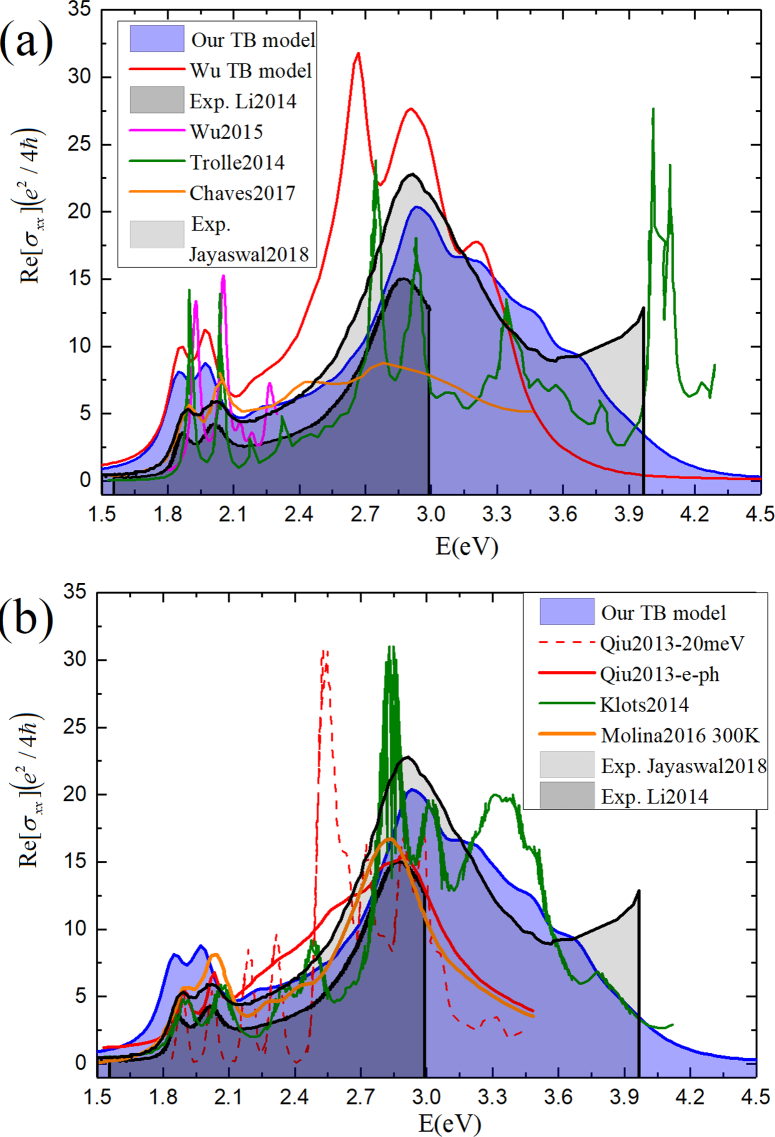
\includegraphics[width=0.35\textwidth]{fig7.png}
\caption{（原文 FIG.~7）不同理论预言的 MoS$_2$ 光学电导率与 Li 及其合作者 [27]、
Jayaswal 及其合作者 [88] 的实验结果比较。
(a) 文献 [11,13,15] 中基于紧束缚的 BSE 解给出的 $\operatorname{Re}(\sigma_{xx})$，
与我们分别基于 Ridolfi 等人 [59] 的紧束缚模型（蓝色）
和 Wu 等人 [13] 的模型（红色）的计算对比
（后者我们加了与图 4 相同的展宽；该曲线需整体移动 $+0.57$~eV 才能与 A、B 激子的实验位置相符 [13]）。
(b) 文献 [10,31,61] 中完全从头算 BSE 解给出的 $\operatorname{Re}(\sigma_{xx})$。
由于后两者 [31,61] 以任意单位给出 $\operatorname{Re}(\sigma_{xx})$，
我们对每条曲线做了纵向缩放以便与实验曲线直接比较。文献 [61] 的曲线取自 300~K。}
\label{fig:7}
\end{figure}

\subsection*{2. 导带条数}

文献 [10] 报道 C 峰由六个近似简并的激子态贡献，
它们来自最高两条价带与最低三条导带（含自旋）之间的跃迁。
图 8 中我们计算了 $N_c=2$、$N_c=6$ 与 $N_c=8$ 下的 $\operatorname{Re}\sigma_{xx}$，
并验证了至少需要 $N_c=6$ 条导带。
可以注意到，正是在 C 激子的能区，两个紧束缚模型的光学电导率都因能带条数增加而获得显著修正。
在 Wu 等人 [13] 的模型中，从 $N_c=6$ 增到 8 时 C 峰还略有增强；
而在我们的紧束缚模型中，最显著的变化发生在由 2 增到 6 时。

\begin{figure}[H]
\centering
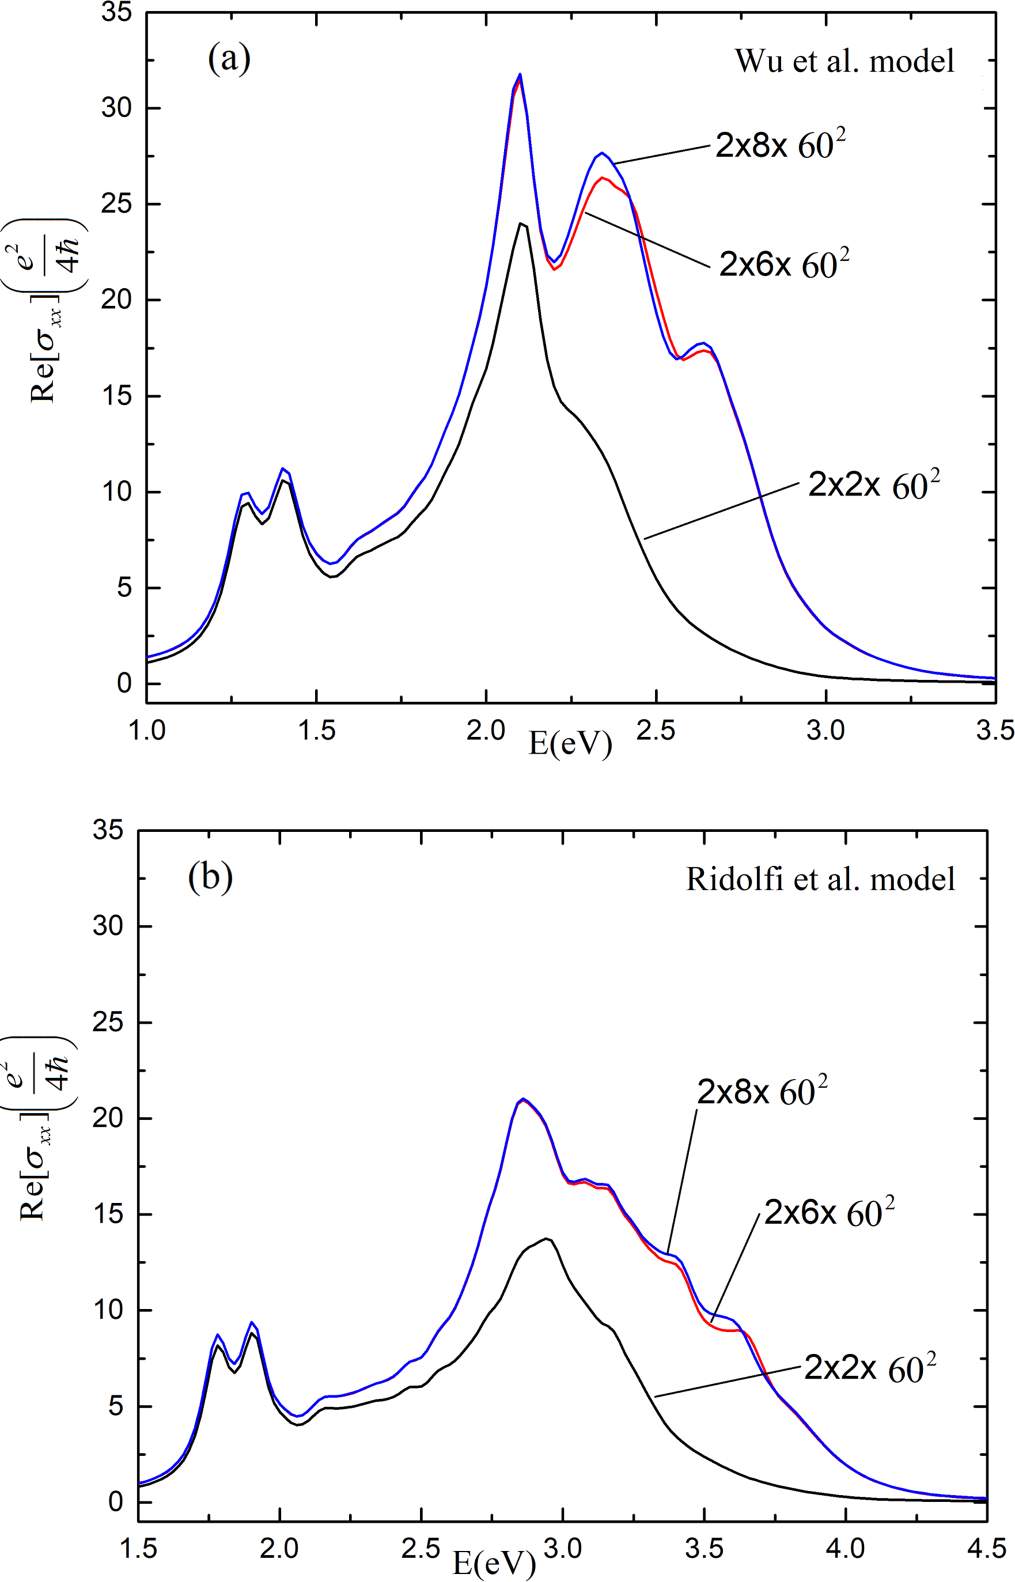
\includegraphics[width=0.42\textwidth]{fig8.png}
\caption{（原文 FIG.~8）采用 Wu 等人 [13]（a）与 Ridolfi 等人 [59]（b）的紧束缚参数化时，
不同导带条数下的线性光学电导率。}
\label{fig:8}
\end{figure}

\subsection*{3. 偶宇称与奇宇称能带}

关于包含过渡金属离子的水平面的镜面对称，对 MoS$_2$ 单层的能带结构有重要影响。
我们用来描述基态能带结构的紧束缚模型 [59] 预言，
在费米能附近有一条偶宇称价带、两条偶宇称导带与两条奇宇称导带（见图 1(a)）。
奇宇称能带的重要性此前并不清楚 [10]，下面我们考察这个问题。
图 9(a) 表明文献 [13] 紧束缚模型中的奇宇称能带对光学电导率没有贡献。
这在预期之内，因为该紧束缚模型不含自旋翻转项：
偶极耦合在自旋空间是对角的，非零跃迁矩阵元必须涉及在该镜面反射下宇称相同的初末态。
我们的紧束缚模型由于哈密顿量中自旋翻转项把奇、偶能带耦合起来，
在“全偶宇称”与“奇偶皆含”两个基组之间只给出很小的差别。
我们由此得出结论：增加能带条数带来的光学电导率增量主要来自上面两条“偶宇称”能带。

\begin{figure}[H]
\centering
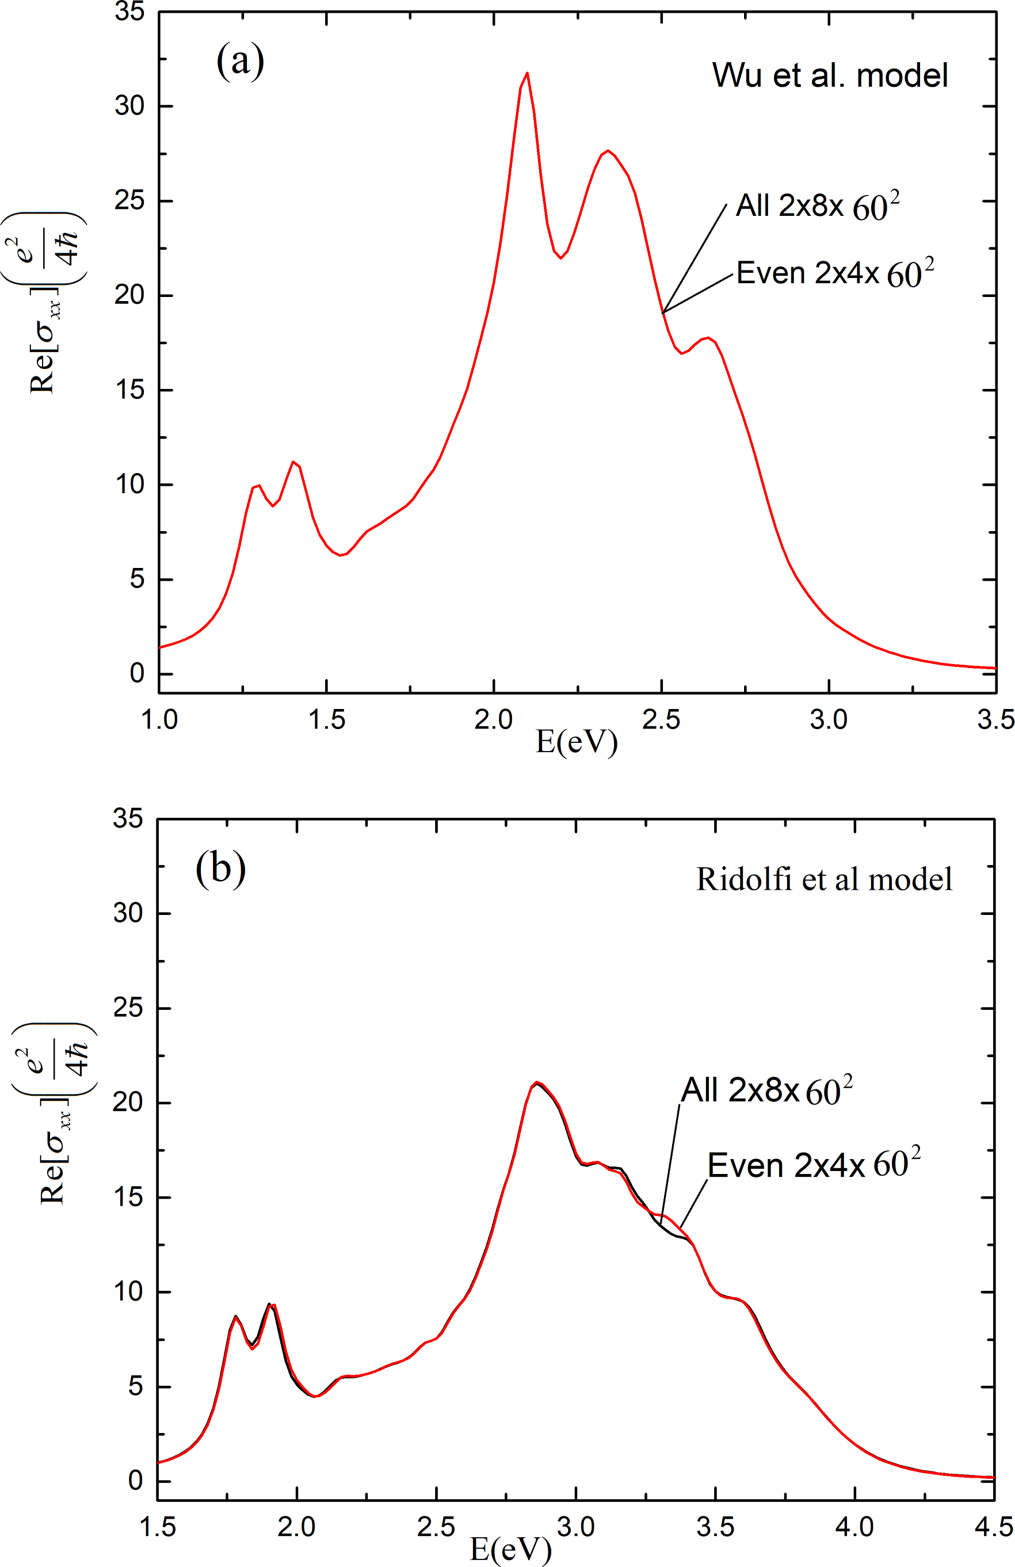
\includegraphics[width=0.42\textwidth]{fig9.png}
\caption{（原文 FIG.~9）采用 Wu 等人 [13]（a）与 Ridolfi 等人 [59]（b）的紧束缚参数化时，
“全能带”模型（$N_c=8$，$N_v=2$，$N_k=60$）与“仅偶宇称能带”模型（$N_c=4$，$N_v=2$，$N_k=60$）
给出的线性光学电导率对比。}
\label{fig:9}
\end{figure}

在解释 C 激子相关谱重转移的来源时，
分析激发谱本身在库仑相互作用下如何变化是有益的。
图 10(a) 给出与图 4 相同的 $\operatorname{Re}\sigma(\omega)$ 数据，
但采用小得多的展宽，以便更清楚地显现精细谱结构。
图 10(b) 比较了含与不含相互作用时的联合态密度（JDOS）。
除带隙中出现束缚激子态之外，可以看到激发谱在很大程度上保持了单电子层面计算的 JDOS。
相互作用造成约 0.1~eV 的全局红移，远小于电导率中所见的谱重转移。
该图还给出了全部激子能级的逆参与比（IPR，式 (A1)），
它定量刻画了相应波函数在倒空间中的局域程度。

\begin{figure}[H]
\centering
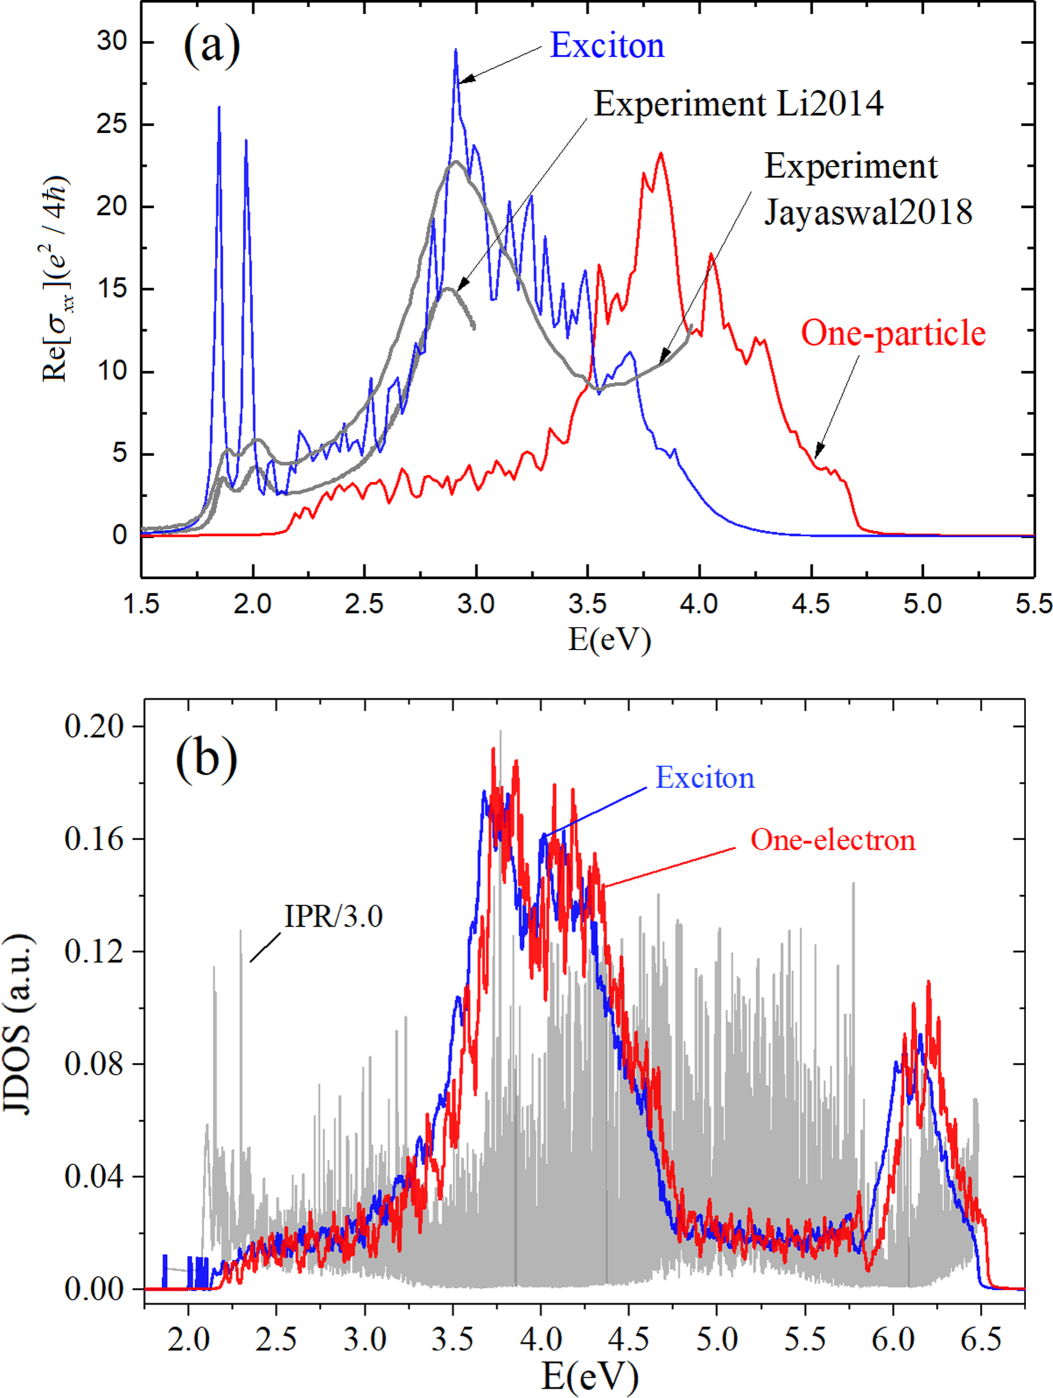
\includegraphics[width=0.5\textwidth]{fig10.png}
\caption{（原文 FIG.~10）(a) 与图 4 相同，但计算曲线改用更小的展宽 0.03~eV（全宽）。
(b) 按式 (18) 定义的激子联合态密度（JDOS）。
所用洛伦兹展宽全宽为 0.01~eV，但在低能区取 0.001~eV 以便分辨单个束缚激子能级。
逆参与比（IPR）按式 (A1) 计算，未作任何展宽。}
\label{fig:10}
\end{figure}

\subsection*{4. 激子逆参与比}

为了对各激子波函数的局域程度获得整体认识，我们对 BSE (5) 的全部本征函数计算了逆参与比（IPR），
\begin{equation}
P(E_M)\equiv\frac{\sum_{cv\mathbf k}\left|A^{M}_{cv\mathbf k}\right|^4}
{\left(\sum_{cv\mathbf k}\left|A^{M}_{cv\mathbf k}\right|^2\right)^2}.
\tag{A1}
\end{equation}
该量粗略度量能量为 $E_M$ 的激子波函数（在倒空间中）的展宽：
最局域的态取值最大，而在整个布里渊区均匀扩展的态按 $\propto1/N_{\mathrm{tot}}$ 标度。
结果已包含在图 10(b) 中。
它表明，一方面 C 激子区域的 JDOS 相对较小，
另一方面该区域的态通常比平均更局域，这从 $[2.75,3.25]$~eV 区间内 IPR 的若干峰可以看出。
这正好反映了从图 5 所选波函数推断出的结论，
并进一步证实我们先前的论断：C 激子在倒空间中比束缚激子局域得多，
即 $P(E\approx E_{A,B})\ll P(E\approx E_C)$。
这当然在预期之内，因为后者在实空间中是真正的束缚态
（与此相关，注意纯 Bloch 态的 $P(\eps_{\mathbf k})=1$，其波函数完全局域在布里渊区的 $\mathbf k$ 点上）。

%=====================================================================
\begin{thebibliography}{99}

\bibitem{r1} Q. H. Wang, K. Kalantar-Zadeh, A. Kis, J. N. Coleman, and M. S. Strano, Nat. Nanotech. 7, 699 (2012).

\bibitem{r2} A. K. Geim and I. V. Grigorieva, Nature (London) 499, 419 (2013).

\bibitem{r3} S. Z. Butler, S. M. Hollen, L. Cao, Y. Cui, J. A. Gupta, H. R. Gutiérrez, T. F. Heinz, S. S. Hong, J. Huang, A. F. Ismach, E. Johnston-Halperin, M. Kuno, V. V. Plashnitsa, R. D. Robinson, R. S. Ruoff, S. Salahuddin, J. Shan, L. Shi, M. G. Spencer, M. Terrones, W. Windl, and J. E. Goldberger, ACS Nano 7, 2898 (2013).

\bibitem{r4} W. Choi, N. Choudhary, G. H. Han, J. Park, D. Akinwande, and Y. H. Lee, Mater. Today 20, 116 (2017).

\bibitem{r5} G. Wang, A. Chernikov, M. M. Glazov, T. F. Heinz, X. Marie, T. Amand, and B. Urbaszek, Rev. Mod. Phys. 90, 021001 (2018).

\bibitem{r6} H.-P. Komsa and A. V. Krasheninnikov, Phys. Rev. B 86, 241201 (2012).

\bibitem{r7} G. Berghäuser and E. Malic, Phys. Rev. B 89, 125309 (2014).

\bibitem{r8} A. Molina-Sánchez, D. Sangalli, K. Hummer, A. Marini, and L. Wirtz, Phys. Rev. B 88, 045412 (2013).

\bibitem{r9} T. C. Berkelbach, M. S. Hybertsen, and D. R. Reichman, Phys. Rev. B 88, 045318 (2013).

\bibitem{r10} D. Y. Qiu, F. H. da Jornada, and S. G. Louie, Phys. Rev. Lett. 111, 216805 (2013).

\bibitem{r11} M. L. Trolle, G. Seifert, and T. G. Pedersen, Phys. Rev. B 89, 235410 (2014).

\bibitem{r12} C. Zhang, A. Johnson, C.-L. Hsu, L.-J. Li, and C.-K. Shih, Nano Lett. 14, 2443 (2014).

\bibitem{r13} F. Wu, F. Qu, and A. H. MacDonald, Phys. Rev. B 91, 075310 (2015).

\bibitem{r14} P. San-Jose, V. Parente, F. Guinea, R. Roldán, and E. Prada, Phys. Rev. X 6, 031046 (2016).

\bibitem{r15} A. J. Chaves, R. M. Ribeiro, T. Frederico, and N. M. R. Peres, 2D Mater. 4, 025086 (2017).

\bibitem{r16} M. Trushin, M. O. Goerbig, and W. Belzig, J. Phys.: Conf. Ser. 864, 012033 (2017).

\bibitem{r17} M. Selig, G. Berghäuser, A. Raja, P. Nagler, C. Schüller, T. F. Heinz, T. Korn, A. Chernikov, E. Malic, and A. Knorr, Nat. Commun. 7, 13279 (2016).

\bibitem{r18} Z. Wang, Y. Xiao, W. Li, R.-Z. Li, and Z.-Q. Li, arXiv:1701.00559.

\bibitem{r19} M. Grüning and C. Attaccalite, Phys. Rev. B 89, 081102 (2014).

\bibitem{r20} M. M. Glazov, L. E. Golub, G. Wang, X. Marie, T. Amand, and B. Urbaszek, Phys. Rev. B 95, 035311 (2017).

\bibitem{r21} S. H. Rhim, Y. S. Kim, and A. J. Freeman, Appl. Phys. Lett. 107, 241908 (2015).

\bibitem{r22} C.-Y. Wang and G.-Y. Guo, J. Phys. Chem. C 119, 13268 (2015).

\bibitem{r23} K. F. Mak, C. Lee, J. Hone, J. Shan, and T. F. Heinz, Phys. Rev. Lett. 105, 136805 (2010).

\bibitem{r24} A. Splendiani, L. Sun, Y. Zhang, T. Li, J. Kim, C.-Y. Chim, G. Galli, and F. Wang, Nano Lett. 10, 1271 (2010).

\bibitem{r25} Y. Li, Y. Rao, K. F. Mak, Y. You, S. Wang, C. R. Dean, and T. F. Heinz, Nano Lett. 13, 3329 (2013).

\bibitem{r26} C. Zhang, H. Wang, W. Chan, C. Manolatou, and F. Rana, Phys. Rev. B 89, 205436 (2014).

\bibitem{r27} Y. Li, A. Chernikov, X. Zhang, A. Rigosi, H. M. Hill, A. M. van der Zande, D. A. Chenet, E.-M. Shih, J. Hone, and T. F. Heinz, Phys. Rev. B 90, 205422 (2014). 4. Exciton and one-electron JDOS

\bibitem{r28} K. P. Dhakal, D. L. Duong, J. Lee, H. Nam, M. Kim, M. Kan, Y. H. Lee, and J. Kim, Nanoscale 6, 13028 (2014).

\bibitem{r29} J. A. Miwa, S. Ulstrup, S. G. Sørensen, M. Dendzik, A. G. Čabo, M. Bianchi, J. V. Lauritsen, and P. Hofmann, Phys. Rev. Lett. 114, 046802 (2015).

\bibitem{r30} H. M. Hill, A. F. Rigosi, C. Roquelet, A. Chernikov, T. C. Berkelbach, D. R. Reichman, M. S. Hybertsen, L. E. Brus, and T. F. Heinz, Nano Lett. 15, 2992 (2015).

\bibitem{r31} A. R. Klots, A. K. M. Newaz, B. Wang, D. Prasai, H. Krzyzanowska, J. Lin, D. Caudel, N. J. Ghimire, J. Yan, B. L. Ivano, K. A. Velizhanin, A. Burger, D. G. Mandru, N. H. Tolk, S. T. Pantelides, and K. I. Bolotin, Sci. Rep. 4, 6608 (2014).

\bibitem{r32} A. F. Rigosi, H. M. Hill, K. T. Rim, G. W. Flynn, and T. F. Heinz, Phys. Rev. B 94, 075440 (2016).

\bibitem{r33} S. H. Aleithan, M. Y. Livshits, S. Khadka, J. J. Rack, M. E. Kordesch, and E. Stinaff, Phys. Rev. B 94, 035445 (2016).

\bibitem{r34} M.-H. Chiu, C. Zhang, H.-W. Shiu, C.-P. Chuu, C.-H. Chen, C.-Y. S. Chang, C.-H. Chen, M.-Y. Chou, C.-K. Shih, and L.-J. Li, Nat. Commun. 6, 7666 (2015).

\bibitem{r35} N. Kumar, S. Najmaei, Q. Cui, F. Ceballos, P. M. Ajayan, J. Lou, and H. Zhao, Phys. Rev. B 87, 161403 (2013).

\bibitem{r36} D. J. Clark, V. Senthilkumar, C. T. Le, D. L. Weerawarne, B. Shim, J. I. Jang, J. H. Shim, J. Cho, Y. Sim, M.-J. Seong, S. H. Rhim, A. J. Freeman, K.-H. Chung, and Y. S. Kim, Phys. Rev. B 90, 121409 (2014).

\bibitem{r37} E. Mishina, N. Sherstyuk, S. Lavrov, A. Sigov, A. Mitioglu, S. Anghel, and L. Kulyuk, Appl. Phys. Lett. 106, 131901 (2015).

\bibitem{r38} M. L. Trolle, Y.-C. Tsao, K. Pedersen, and T. G. Pedersen, Phys. Rev. B 92, 161409 (2015).

\bibitem{r39} A. Säynätjoki, L. Karvonen, H. Rostami, A. Autere, S. Mehravar, A. Lombardo, R. A. Norwood, T. Hasan, N. Peyghambarian, H. Lipsanen, K. Kieu, A. C. Ferrari, M. Polini, and Z. Sun, Nat. Commun. 8, 893 (2016).

\bibitem{r40} R. I. Woodward, R. T. Murray, C. F. Phelan, R. E. P. de Oliveira, T. H. Runcorn, E. J. R. Kelleher, S. Li, E. C. de Oliveira, G. J. M. Fechine, G. Eda, and C. J. S. de Matos, 2D Mater. 4, 011006 (2017).

\bibitem{r41} X. Yin, Z. Ye, D. A. Chenet, Y. Ye, K. O’Brien, J. C. Hone, and X. Zhang, Science 344, 488 (2014).

\bibitem{r42} S. Zhang, N. Dong, N. McEvoy, M. O’Brien, S. Winters, N. C. Berner, C. Yim, Y. Li, X. Zhang, Z. Chen, L. Zhang, G. S. Duesberg, and J. Wang, ACS Nano 9, 7142 (2015).

\bibitem{r43} F. Liu, J. Zhou, C. Zhu, and Z. Liu, Adv. Funct. Mater. 27, 1602404 (2017).

\bibitem{r44} Y. Saito, T. Nojima, and Y. Iwasa, Supercond. Sci. Technol. 29, 93001 (2016).

\bibitem{r45} F. Wang, Z. Wang, Q. Wang, F. Wang, L. Yin, K. Xu, Y. Huang, and J. He, Nanotechnology 26, 292001 (2015).

\bibitem{r46} A. Raja, A. Chaves, G. A. Jaeeun Yu, H. M. Hill, A. F. Rigosi, T. C. Berkelbach, P. Nagler, C. Schüller, T. Korn, C. Nuckolls, J. Hone, L. E. Brus, T. F. Heinz, D. R. Reichman, and A. Chernikov, Nat. Commun. 8, 15251 (2017).

\bibitem{r47} S. Nakajima, Y. Toyozawa, and R. Abe, The Physics of Elementary Excitations (Springer-Verlag, Berlin, New York, 1980).

\bibitem{r48} R. Roldán, L. Chirolli, E. Prada, J. A. Silva-Guillén, P. San-Jose, and F. Guinea, Chem. Soc. Rev. 46, 4387 (2017).

\bibitem{r49} M. Ugeda, A. Bradley, S.-F. Shi, F. H. da Jornada, Y. Zhang, D. Qiu, W. Ruan, S. Mo, Z. Hussain, Z.-X. Shen, F. Wang, S. Louie, and M. Crommie, Nat. Mater. 13, 1091 (2014).

\bibitem{r50} D. Xiao, G.-B. Liu, W. Feng, X. Xu, and W. Yao, Phys. Rev. Lett. 108, 196802 (2012).

\bibitem{r51} K. F. Mak, K. He, J. Shan, and T. F. Heinz, Nat. Nanotech. 7, 494 (2012).

\bibitem{r52} H. Zheng, J. Dai, W. Yao, D. Xiao, and X. Cui, Nat. Nanotech. 7, 490 (2012).

\bibitem{r53} G. Sallen, L. Bouet, X. Marie, G. Wang, C. R. Zhu, W. P. Han, Y. Lu, P. H. Tan, T. Amand, B. L. Liu, and B. Urbaszek, Phys. Rev. B 86, 081301 (2012).

\bibitem{r54} T. Cao, G. Wang, W. Han, H. Ye, C. Zhu, J. Shi, Q. Niu, P. Tan, E. Wang, B. Liu, and J. Feng, Nat. Commun. 3, 887 (2012).

\bibitem{r55} L. Bawden, S. P. Cooil, F. Mazzola, J. M. Riley, L. J. CollinsMcIntyre, V. Sunko, K. W. B. Hunvik, M. Leandersson, C. M. Polley, T. Balasubramanian, T. K. Kim, M. Hoesch, J. W. Wells, G. Balakrishnan, M. S. Bahramy, and P. D. C. King, Nat. Commun. 7, 11711 (2016).

\bibitem{r56} J. Zhou, W. Y. Shan, W. Yao, and D. Xiao, Phys. Rev. Lett. 115, 166803 (2015).

\bibitem{r57} A. Srivastava and A. Imamoğlu, Phys. Rev. Lett. 115, 166802 (2015).

\bibitem{r58} M. Rohlfing and S. G. Louie, Phys. Rev. B 62, 4927 (2000).

\bibitem{r59} E. Ridolfi, D. Le, T. S. Rahman, E. R. Mucciolo, and C. H. Lewenkopf, J. Phys.: Condens. Matter 27, 365501 (2015).

\bibitem{r60} A. Ramasubramaniam, Phys. Rev. B 86, 115409 (2012).

\bibitem{r61} A. Molina-Sánchez, M. Palummo, A. Marini, and L. Wirtz, Phys. Rev. B 93, 155435 (2016).

\bibitem{r62} S. Tongay, J. Zhou, C. Ataca, K. Lo, T. S. Matthews, J. Li, J. C. Grossman, and J. Wu, Nano Lett. 12, 5576 (2012).

\bibitem{r63} G. Kioseoglou, A. Hanbicki, M. Currie, A. Friedman, and B. Jonker, Sci. Rep. 6, 25041 (2016).

\bibitem{r64} For example, Ref. [10] attributes the peak C to transitions near, but not directly at, the $\Gamma$ point, which require a fine sampling with 3002 k points and at least 56 bands in the underlying GW calculation. The authors also use local field effects to include the interaction over different BZs.

\bibitem{r65} P. Cudazzo, I. V. Tokatly, and A. Rubio, Phys. Rev. B 84, 085406 (2011).

\bibitem{r66} A. Chernikov, T. C. Berkelbach, H. M. Hill, A. Rigosi, Y. Li, O. B. Aslan, D. R. Reichman, M. S. Hybertsen, and T. F. Heinz, Phys. Rev. Lett. 113, 076802 (2014).

\bibitem{r67} A. S. Rodin, A. Carvalho, and A. H. Castro Neto, Phys. Rev. B 90, 075429 (2014).

\bibitem{r68} L. V. Keldysh, JETP Lett. 29, 658 (1979).

\bibitem{r69} N. Saigal, V. Sugunakar, and S. Ghosh, Appl. Phys. Lett. 108, 132105 (2016).

\bibitem{r70} E. E. Salpeter and H. A. Bethe, Phys. Rev. 84, 1232 (1951).

\bibitem{r71} http://www.bethe-salpeter.org.

\bibitem{r72} S. Albrecht, L. Reining, R. Del Sole, and G. Onida, Phys. Rev. Lett. 80, 4510 (1998).

\bibitem{r73} J. Li, M. Holzmann, I. Duchemin, X. Blase, and V. Olevano, Phys. Rev. Lett. 118, 163001 (2017).

\bibitem{r74} G. Grosso and G. P. Parravicini, Solid State Physics (Oxford, Elsevier Science, 2014).

\bibitem{r75} For the derivation of the BSE in details on the computation of W see, for instance, Chaps. VII.1. and IV.4-5 of Ref. [74].

\bibitem{r76} S. Latini, T. Olsen, and K. S. Thygesen, Phys. Rev. B 92, 245123 (2015).

\bibitem{r77} The expression $r_0=\varepsilon_2 d/(\varepsilon_1+\varepsilon_3)$ is sometimes reported as the limit of Eq. (10) when $\varepsilon_2\gg\varepsilon_{1,3}$.

\bibitem{r78} F. M. Hipolito, On linear and non-linear interactions of light with two dimensional materials, Ph.D. thesis, National University of Singapore 2016.

\bibitem{r79} Having α1 = 1,α2,3 = 0 in Eq. (17) corresponds to leaving the factor ∝1/κ(q) in the potential (8) outside of the average integral.

\bibitem{r80} Recall that if Nk = 100, the full diagonalization of the BSE Hamiltonian requires handling a matrix of dimension Ntot × Ntot = (104 Nc Nv )2 . For us, with Nc = 8 and Nv = 2, that amounts to ≃ 2.56 × 1010 .

\bibitem{r81} In particular, \#11 consists of choosing q = 0 at the center of a square integration domain of side 2π /aNk and \#2 in placing q = 0 at the corner of the same integration square.

\bibitem{r82} M. R. Molas, C. Faugeras, A. O. Slobodeniuk, K. Nogajewski, M. Bartos, D. M. Basko, and M. Potemski, 2D Mater. 4, 021003 (2017).

\bibitem{r83} J. P. Echeverry, B. Urbaszek, T. Amand, X. Marie, and I. C. Gerber, Phys. Rev. B 93, 121107(R) (2016).

\bibitem{r84} M. Baranowski, A. Surrente, D. K. M. M. Ballottin, A. Mitioglu, P. Christianen, Y. Kung, D. Dumcenco, A. Kis, and P. Plochocka, 2D Mater. 4, 025016 (2017).

\bibitem{r85} E. Malic, M. Selig, M. Feierabend, S. Brem, D. Christiansen, F. Wendler, A. Knorr, and G. Berghäuser, Phys. Rev. Mater. 2, 014002 (2018).

\bibitem{r86} X. Zhang, T. Cao, Z. Lu, Y. Lin, F. Zhang, Y. Wang, Z. Li, J. Hone, J. Robinson, D. Smirnov, S. Louie, and T. F. Heinz, Nat. Nanotech. 12, 883 (2017).

\bibitem{r87} Alternatively, the experimental positions of the A and B peaks can be matched by tuning the environment dielectric constants that determine r0 [cf. Eq. (10)] [11].

\bibitem{r88} G. Jayaswal, Z. Dai, X. Zhang, M. Bagnarol, A. Martucci, and M. Merano, Opt. Lett. 43, 703 (2018).

\bibitem{r89} The results for the B excitons are not shown explicitly but are similar to those reported in Fig. 5 for the A counterparts.

\bibitem{r90} A. Molina-Sánchez, K. Hummer, and L. Wirtz, Surf. Sci. Rep. 70, 554 (2015).

\bibitem{r91} At a technical level, it is important to realize that the sharp localization associated with the C excitons requires a fine k-point mesh to ensure proper convergence of the absorption spectrum over this large range of energies 10.

\bibitem{r92} L. M. Malard, T. V. Alencar, A. P. M. Barboza, K. F. Mak, and A. M. de Paula, Phys. Rev. B 87, 201401 (2013).

\bibitem{r93} E. Cappelluti, R. Roldán, J. A. Silva-Guillén, P. Ordejón, and F. Guinea, Phys. Rev. B 88, 075409 (2013).

\bibitem{r94} We stress, however, that some models require rather large rigid shifts in energy and/or vertical scaling in order to make the calculated results agree with the experimental traces as shown in Fig. 7.

\bibitem{r95} For completeness, it is worth noting that the spectral shape in the range of the C excitons measured in MoS2 multilayers changes appreciably with layer number, as shown by the experiments reported in Ref. [28].
\end{thebibliography}

\end{document}
